\documentclass[12pt,a4paper,twoside,openright]{book}
\usepackage[T1]{fontenc}
\usepackage[utf8]{inputenc}
\usepackage{microtype}
\usepackage[italian,english]{babel}
\usepackage[binding=5mm]{layaureo}
\usepackage[suftesi]{frontespizio}
\usepackage{emptypage}
\usepackage{indentfirst}
\usepackage{booktabs}
\usepackage{tabularx}
\usepackage{graphicx}
\usepackage{subfigure}
\usepackage{caption}
\usepackage{listings}
\usepackage{amsmath,amssymb,amsthm,mathtools}
\usepackage{mparhack,fixltx2e,relsize}
\usepackage{chngpage,calc}
\usepackage{xcolor}
\usepackage{braket}
\usepackage{slashed}
\usepackage{bbold}
\usepackage{physics}
\usepackage{tikz}
\usepackage{tikz-cd}

%%%%%%%%%%%%%%%%%%%%%%%%%%%%%%%%%%%%%%%%%%%%%%%%

%\DeclarePairedDelimiter{\abs}{\lvert}{\rvert}
%TRACE
%\newcommand{\tr}{\mathrm {Tr}}
%IDENTITY MATRIX
\newcommand{\id}{\mathbb{1}}
%REAL-IMAGINARY PART
\newcommand{\re}{ \mathrm{Re}}
\newcommand{\im }{ \mathrm{Im }}
%SU(2) LEFT
\newcommand{ \suEW}{SU(2)$_L$ }
%DERIVATIVE
\newcommand{ \der}[2]{\frac{\mathrm{d} #1}{\mathrm{d} #2}}
%IN-LINE DERIVATIVE
\newcommand{ \ILder}[2]{\mathrm{d} #1 / \mathrm{d} #2}
%PARTIAL DERIVATIVE
\newcommand{ \pder}[2]{\frac{\partial #1}{\partial #2}}
%FUNCTIONAL INTEGRATION MEASURE
\newcommand{\D}{\mathcal D}
%LAGRANGIAN
\newcommand{\Lag}{\mathcal L}
%d^4x
\newcommand{\dx}{\mathrm{d}^4x }

%FUNDAMENTAL REPRESENTATION
\def\drawbox#1#2{\hrule height#2pt
        \hbox{\vrule width#2pt height#1pt \kern#1pt
              \vrule width#2pt}
              \hrule height#2pt}
\def\Fund#1#2{\vcenter{\vbox{\drawbox{#1}{#2}}}}
\def\fund{\Fund{6.4}{0.3}}


%%%%%%%%%%%%%%%%%%%%%%%%%%%%%%%%%%%%%%%%%%%%%%%%

\pagestyle{plain}

\begin{document}

\frontmatter

\chapter*{Abstract}

In this thesis we present two quite different studies, having as a common theme non-Abelian gauge theories applied to Beyond the Standard Model physics. The first is a non-perturbative analysis, performed with lattice techniques, of an SU(2) gauge theory with fundamental fermion and scalar fields. The results of this study are relevant in the context of composite Higgs models based on the recently proposed mechanism of fundamental partial compositeness. The second study concerns the transport coefficients of gauge theories featuring large-distance conformality. This study addresses the important topic of the thermodynamic properties of theories in the conformal window, and inspects the applicability of perturbative results for transport coefficients to this class of theories.


\tableofcontents

\chapter{Introduction}

This thesis has as a common topic non-Abelian gauge theories applied to Beyond the Standard Model physics.
The Standard Model of particle physics is very successful in describing experimental data. Nevertheless, we know that it is just an effective theory, valid only up to an ultraviolet cutoff. 
The question of what kind of new physics may constitute extensions of the Standard Model is very fascinating, and it occupies a consistent part of the high-energy-physics community. 
In this thesis, we consider two deeply related topics belonging to Beyond the Standard Model research: the first is composite Higgs models and the second the conformal window.
Composite Higgs models address the question of mass generation, and aim at providing a more theoretically consistent framework with respect to the Standard Model Higgs mechanism. 
In order to build phenomenologically viable composite Higgs models, gauge theories with a "walking" coupling are needed. These theories have an approximate infrared fixed point, and are found in theory space close to the lower boundary of the so-called conformal window. Theories in the conformal window display large-distance conformality, due to an infrared fixed point in the renormalisation group flow of the gauge coupling.

In this thesis we present a lattice study of the SU(2) gauge theory with two fundamental fermion flavours and one fundamental scalar field. This model is intended as a minimal scenario for testing the non-perturbative dynamics of recently proposed models of  fundamental partial compositeness \cite{Sannino:2016sfx}. These are composite Higgs models featuring fermionic and scalar matter fields, which are able to provide a complete theory of flavour, alternative to the Standard Model Higgs mechanism. 
The second study presented in this thesis regards the thermodynamic properties of theories in the conformal window. In particular, we study the transport coefficients of theories in the perturbative conformal window.

This thesis is organised as follows: in chapter \ref{LFT}, we give a general introduction to lattice field theory, mostly focused on the tools needed for the lattice study presented in this thesis. In chapter \ref{GFS}, after introducing composite Higgs models and the fundamental partial compositeness mechanism, we present the results of our lattice study of the SU(2) gauge theory with two fundamental fermions and one fundamental scalar. In chapter \ref{CW}, we present our study of the transport coefficients of theories in the conformal window. Before discussing our results, we provide the definitions of the transport coefficients under analysis, and we describe the method used by the authors of \cite{Arnold:2000dr} to obtain perturbative estimates of the transport coefficients of a hot gauge theory, which constitute the basis of our computations.
In appendix, some general definitions and additional material can be found.

\mainmatter


\chapter{The standard model of particle physics}



%%%%%%%%%%%%%%%%%%%%%%%%%%%%%%%%%%%%%%%%%%%%%%%%%%%%%%

\section{Gauge symmetry}


%%%%%%%%%%%%%%%%%%%%%%%%%%%%%%%%%%%%%%%%%%%%%%%%%%%%%%

\section{Electroweak and strong interactions}


%%%%%%%%%%%%%%%%%%%%%%%%%%%%%%%%%%%%%%%%%%%%%%%%%%%%%%

\section{Electroweak symmetry breaking}


%%%%%%%%%%%%%%%%%%%%%%%%%%%%%%%%%%%%%%%%%%%%%%%%%%%%%%

\section{On the spontaneous breaking of gauge symmetries}



%%%%%%%%%%%%%%%%%%%%%%%%%%%%%%%%%%%%%%%%%%%%%%%%%%%%%%

\chapter{Lattice field theory}
\label{LFT}

In an interacting quantum field theory, controllable analytical computations can only be performed in perturbation theory, i.e. the coupling constants are assumed to be small, so that the interactions represent a small perturbation of the free-field Lagrangian. A large class of non-Abelian gauge theories (among which QCD) is strongly coupled at low energies. This implies that the large-distance properties of these theories cannot be computed in perturbation theory. 

Lattice field theory is a non-perturbative tool for studying quantum field theories, and it is therefore very valuable in the context of strongly coupled theories. In this chapter, we give a general introduction to lattice field theory, focusing mainly on the tools needed for the lattice study described in this thesis. The chapter is organised as follows: we start by introducing Monte Carlo simulations, a numerical tool of statistical mechanics, which can be applied to quantum field theories defined in Euclidean space. 
We then discuss the lattice discretisation of the action of a gauge theory coupled to fermions. We continue by describing the Hybrid Monte Carlo algorithm, which is used for the lattice analysis presented in this thesis. Then we give a short introduction to the topic of mass measurements on the lattice, and we conclude by discussing the continuum limit of lattice theories.


%%%%%%%%%%%%%%%%%%%%%%%%%%%%%%%%%%%%%%%%%%%%%%%%%%%%%%

\section{Quantum field theory and statistical mechanics}
\label{QFT-SM}

We can build a non-perturbative tool for quantum field theory by exploiting the strong similarity between quantum field theory and statistical mechanics. This gives us the possibility of applying Monte Carlo simulations, an intrinsically non-perturbative method, to quantum field theory.

In the path-integral formulation of quantum field theory, the generating functional of correlation functions is defined as:
\begin{equation}
Z[J] = \int \D \phi \exp \biggl[ i \int \dx \: \bigl( \Lag[\phi] + J(x)\phi(x) \bigr) \biggr] \: ,
\label{QFT_generator}
\end{equation}
%
where $\phi$ generically represents the field content of the theory, $\Lag$ is the Lagrangian and $J(x)$ is an external source field. $n$-point functions are obtained by applying the functional derivative $\delta / \delta J(x)$ to $Z[J]$ as follows:
\begin{equation}
\begin{split}
\bra{0} \mathrm T \phi(x_1) \dots \phi(x_n) \ket{0} = & \frac{1}{Z[0]} \prod_{i=1}^n \biggl( -i \frac{\delta}{\delta J(x_i)} \biggr) Z[J] \biggr\vert_{J=0} = \\
& = \frac{1}{Z[0]} \int \D \phi \: \phi(x_1) \dots \phi(x_n) \exp \biggl[ i \int \dx \: \Lag[\phi] \biggr] \; ,
\end{split}
\label{np_function}
\end{equation}
%
where $\ket{0}$ represents the vacuum state and T the time-ordered product.
By performing a Wick rotation, we can make the generating functional \ref{QFT_generator} to be formally equal to the partition function of a statistical mechanical model.

As a concrete example, we consider a complex scalar field theory, with action:
\begin{equation}
S[\phi,\phi^*] = \int \dx \: \Lag[\phi,\phi^*] = \int \dx \bigl( \partial_{\mu} \phi^* \partial^{\mu} \phi - m^2 \abs{\phi}^2 -\lambda \abs{\phi}^4 \bigr) \; ,
\end{equation}
%
and generating functional:
\begin{equation}
Z[J,J^*] = \int \D \phi \D \phi^* \exp \biggl[ i S[\phi,\phi^*] + i \int \dx \: J^*(x) \phi(x) + \phi^*(x) J(x) \biggr] \; .
\label{scalar_gen_functional}
\end{equation}
%
After performing a Wick rotation ($x^0 = -i x^0_E$, $x^i = x^i_E$), the following changes occur:
\begin{equation}
\begin{split}
& i\dx =  \dx_E \\
& \partial_{\mu} \phi^* \partial^{\mu} \phi = - \delta_{\mu\nu} \partial^{\mu}_E \phi^* \partial^{\nu}_E \phi \; .
\end{split}
\end{equation}
%
We define the Euclidean action as:
\begin{equation}
S_E[\phi,\phi^*] = \int \dx_E \bigl( \delta_{\mu\nu} \partial^{\mu}_E \phi^* \partial^{\nu}_E \phi + m^2 \abs{\phi}^2 + \lambda \abs{\phi}^4  \bigr) \; ,
\end{equation}
%
and we find that the generating functional
\begin{equation}
Z[J,J^*] = \int \D \phi \D \phi^* \exp \biggl[ - \biggl( S_E[\phi,\phi^*] - \int \dx_E J(x_E) \phi(x_E) - J^*(x_E) \phi^*(x_E) \biggr) \biggr] 
\end{equation}
%
is now formally equal to the partition function of a statistical mechanical system.

%%%%%%%%%%%%%%%%%%%%%%%%%%%%%%%%%%%%%%%%%%%%%%%%%%%%%%

\section{Monte Carlo simulations}

In statistical mechanics, the probability for a system in thermal equilibrium to be found in the microscopical configuration $\phi$ is given by:
\begin{equation}
P[\phi] = \frac{e^{-H[\phi]/k_B T}}{Z} \; ,
\end{equation}
%
$Z=\sum_{\phi} \exp[-H[\phi]/k_B T]$ being the partition function, $H[\phi]$ the total energy of the system in the configuration $\phi$, $k_B$ the Boltzmann constant and $T$ the temperature. Monte Carlo simulations are a numerical method for generating configurations distributed according to the probability distribution $P[\phi]$.

In the previous section, we argued that a quantum field theory, defined by the action $
S[\phi]$, is equivalent to a statistical mechanical model with partition function
\begin{equation}
Z = \int \D \phi \: e^{- S_E[\phi]}
\end{equation}
%
(here for simplicity we consider the case of zero external source). We can apply the Monte Carlo method for generating configurations distributed according to:
\begin{equation}
P[\phi] = \frac{e^{-S_E[\phi]}}{Z} \: .
\label{Boltz_dist}
\end{equation}


Once we have an ensemble of such configurations, $n$-point functions are calculated by averaging products of fields over the configurations:
\begin{equation}
\frac{1}{Z} \int \D \phi \: \phi(x_1) \dots \phi(x_n) e^{ -S_E[\phi]} \longrightarrow \frac{1}{N}\sum_{i=1}^N \phi_i(x_1) \dots \phi_i(x_n) \; ,
\label{n_point_f}
\end{equation}
%
where $\phi_i(x_j)$ is the value of the field $\phi$ at the space-time point $x_j$, in the $i$-th configuration. 


In order to construct a Monte Carlo simulation, we consider a stochastic process generating a sequence of configurations.  We start from an initial configuration $\phi_0$ at "Monte-Carlo time" (MC-time) $t = 0$, and move to a new configuration $\phi_1$ with transition probability $W(\phi_0 \to \phi_1)$. The following normalisation condition holds for the transition probability $W$:
\begin{equation}
\sum_{\phi'} W(\phi \to \phi') = 1 \; .
\label{prob_norm}
\end{equation}
%
We repeat this procedure many times, thus generating a sequence of configurations. The probability $P[\phi; t]$ of being in the configuration $\phi$ at MC-time $t$ fulfils the following condition:
\begin{equation}
P[\phi; t] = \sum_{\phi'} P[\phi'; t-1] W(\phi' \to \phi) \; .
\label{prob_evolution}
\end{equation}

We want the stochastic process to have the Boltzmann distribution $P_B[\phi] = \exp[-S_E[\phi]]/Z$ as an attractive fixed point. This means that the probability distribution $P[\phi; t]$ approaches $P_B[\phi]$ in the limit of large $t$. In practical simulations, after some thermalisation time $t_T$, the probability distribution stops changing with MC-time, and it equals the Boltzmann distribution: $P[\phi; t>t_T] = P_B[\phi]$. If we are able to build such a stochastic process, then we can obtain an ensemble of Boltzmann-distributed configurations on which we can apply equation \ref{n_point_f} for calculating $n$-point functions.

It follows from equation \ref{prob_evolution} that, if $P_B$ is a fixed point of the stochastic process, then:
\begin{equation}
P_B[\phi] = \sum_{\phi'} P_B[\phi'] W(\phi' \to \phi) \; .
\label{fixed_p}
\end{equation}
%
We define the detailed-balance relation as:
\begin{equation}
P_B[\phi] W(\phi \to \phi') = P_B[\phi'] W(\phi' \to \phi) \; ;
\label{detailed_bal}
\end{equation}
%
this relation implies the fixed-point condition \ref{fixed_p} (this can be shown by summing equation \ref{detailed_bal} over $\phi'$, and using the normalisation condition \ref{prob_norm}), and it is easier to verify in a specific stochastic process. A process satisfying the detailed balance relation can be parametrised as follows:
\begin{equation}
W(\phi \to \phi') = F\biggl(\frac{P_B[\phi']}{P_B[\phi]} \biggr) \; ,
\label{F1}
\end{equation}
%
where $F$ is a generic function satisfying the functional equation
\begin{equation}
\frac{F(z)}{F(1/z)} = z \; .
\label{F2}
\end{equation}
%
There are many possible choices for the function $F$, each of whom defines a viable algorithm for a Monte Carlo simulation. One of the most widely used is $F(z) = \min [1,z]$, leading to the transition probability:
\begin{equation}
W(\phi \to \phi') = \min\biggl[1, \frac{P_B[\phi']}{P_B[\phi]}\biggl] = \min\bigl[1,e^{-(S_E[\phi'] - S_E[\phi])}\bigr] \; .
\label{Metropolis}
\end{equation}
%
This particular implementation of the Monte Carlo method is known as Metropolis algorithm \cite{Metropolis:1953am}.

The stochastic process described above can be implemented numerically. To make this possible, we must define the theory on a lattice of finite volume, so that each field configuration is represented by a discrete and finite set of real numbers. Specifically, one configuration is completely defined by the value of each field at each point of the discretised space-time.  In section \ref{Lattice_action} we will discuss the definition of a gauge theory on a space-time lattice.

To conclude, Monte Carlo simulations are a powerful non-perturbative method for studying quantum field theories. The price to be paid is the introduction of different sources of error that must be carefully treated: discretisation errors, finite-volume effects and statistical errors due to conducting the analysis on a finite set of configurations. 




%%%%%%%%%%%%%%%%%%%%%%%%%%%%%%%%%%%%%%%%%%%%%%%%%%%%%%

\section{Lattice action}
\label{Lattice_action}

As previously pointed out, in order to apply the Monte Carlo method to a quantum field theory, we must first define the theory on a discretised space-time. In this section we discuss the lattice discretisation of a gauge theory coupled to fermions.

We define the discretised space-time as the set of points:
\begin{equation}
\Lambda = \set{x_{\mu} = n_{\mu} a  \mid  n_{\mu} = 0, \dots, L_{\mu} -1, \; \mu = 0, \dots, 3 } \; ,
\end{equation}
%
where $a$ is the lattice spacing and $L_{ \mu}$ the number of lattice points in direction $\mu$. We denote by $\hat \mu$ the unit vector in direction $\mu$. As discussed in section \ref{QFT-SM}, we are interested in defining the theory on a Euclidean space-time . However, for some purposes (such as measuring masses via the exponential falloff of correlators) it is useful to maintain the notion of time direction on the lattice. We consider $\mu = 0$ as time direction, i.e. the one that must be Wick-rotated in order to analytically continue the Euclidean theory to Minkowski space.

When we define a quantum field theory on a lattice with a finite number of points, the functional integral becomes the product of a finite number of ordinary integrals. For example, in the case of a real scalar field theory we have:
\begin{equation}
\int \D \phi \to \int_{-\infty}^{\infty} \prod_{x \in \Lambda} \mathrm{d} \phi_x \: ,
\end{equation}
%
where $\phi_x$ is the value of the field $\phi$ at the lattice point $x$.

\subsection{Gauge action}

We consider a theory with SU(N) gauge symmetry, whose continuum action in Euclidean space is defined by:
%
\begin{equation}
S_{YM}^E [A] = \frac{1}{4} \int \dx \bigl(F_{\mu \nu}^a(x)\bigr)^2 \: ,
\label{Yang-Mills-E}
\end{equation}
%
where $A_{\mu}^a$ is the gauge field, and the field strength tensor $F_{\mu\nu}^a$ is defined as follows:
\begin{equation}
F_{\mu\nu}^a = \partial_{\mu} A^a_{\nu} - \partial_{\nu} A^a_{\mu} - g f^{abc} A_{\mu}^b A_{\nu}^c \: .
\end{equation}
%
In this equation, $g$ represents the gauge coupling and $f^{abc}$ the structure constants, defined by:
\begin{equation}
[T^a,T^b] = i f^{abc} T^c \: ,
\end{equation}
%
where $T^a$, $a \in  [1, \dots, \mathrm{N}^2 -1]$, are the generators of the fundamental representation  of  SU(N).
In equation \ref{Yang-Mills-E}, the indices $\mu$, $\nu$, $a$ are summed over.
In order to define a discretised version of this theory, we assign to each link on the lattice $\Lambda$ an element of the gauge group:
\begin{equation}
U_ {\mu}(x) = \exp\biggl[i a  g A^b_{\mu}(x) T^b \biggr] \in \mathrm{SU(N)} \; ,
\label{link_var}
\end{equation}
%
where $g$ is again the gauge coupling. The following relation holds for the link variables $U_{\mu}$:
\begin{equation}
U_{-\mu}(x)  = U_{\mu}(x - a\hat\mu)^{\dagger} \; .
\end{equation}

We define a gauge transformation by assigning to each lattice site an independent element of the gauge group, $\Omega(x) \in \mathrm{SU(N)}$,  and transforming the  link variables as follows:
\begin{equation}
U_ {\mu}(x) \to  U_{\mu}'(x) = \Omega(x) U_{\mu}(x) \Omega(x+  a \hat \mu)^{\dagger} \; .
\label{lattice_GT}
\end{equation}

The  Wilson plaquette action \cite{Wilson:1974sk} is the first proposed lattice discretisation of the  Yang-Mills action. It is defined as:
\begin{equation}
S_W[U] =  \frac{2 \mathrm N}{g^2} \sum_{x \in \Lambda}  \sum_{\mu < \nu} \biggl[  1 - \frac{1}{\mathrm{N}} \re \tr  [U_{\mu \nu}] \biggr] \; ,
\end{equation}
%
where the plaquette $U_{\mu \nu}$ is the ordered product of the link variables around an elementary loop on the lattice:
\begin{equation}
U_{\mu \nu}(x)  = U_{\mu}(x) U_{\nu}(x + a\hat\mu) U_{\mu}(x+\hat\nu)^{\dagger} U_{\nu}(x) ^{\dagger}   \; .
\label{plaquette}
\end{equation}
%
$S_W[U]$ is invariant under the gauge transformation \ref{lattice_GT}, and, in the limit $a \to 0$, it reduces to the Euclidean Yang-Mills action.
This can be shown by expanding the link variables \ref{link_var} in powers of $a$, and by making use of the Baker-Campbell-Hausdorff formula for expanding the products of link variables:
\begin{equation}
e^A e^B = e^{A+B+\frac{1}{2}[A,B] + \dots}
\end{equation}
%
where $A$  and $B$ are generic matrices, and we are omitting higher powers of the matrices in the right-hand side. Moreover, we can relate a finite difference on the lattice to a continuum derivative as follows:

\begin{equation}
A_{\mu}(x + a \hat \nu) - A_{\mu}(x) = a \: \partial_{\nu} A_{\mu}(x) + \mathcal{O}(a^2) \; .
\end{equation}
%
We find:

\begin{equation}
S_W[U] = \frac{a^4}{2} \sum_{x \in \Lambda} \sum_{\mu, \nu} \tr [F_{\mu \nu}(x)^2]  + \mathcal O(a^2) \underset{a \to 0, V \to \infty}{\longrightarrow} \frac{1}{4} \int \dx \: (F_{\mu \nu}^a)^2 = S_{YM}^E[A]\; ,
\end{equation}
%
where $V = \prod_{\mu = 0}^3L_{\mu}$ is the total number of lattice points, and $F_{\mu\nu} = F^a_{\mu\nu} T^a$.

It must be noticed that, as we discretise the Yang-Mills action, the Poincaré symmetry of the continuum theory is reduced to the smaller group of symmetries of an hypercubic lattice. However, the discretised action that we defined has the remarkable property of being exactly gauge invariant even at finite lattice spacing.



\subsection{Fermion action}
\label{fermion_action}

The continuum Dirac action in Euclidean space is defined by:
\begin{equation}
S_D^E[\psi, \bar \psi, A] = \int \dx  \: \bar \psi (\slashed D + m \id) \psi = \int \dx \: \bar \psi \bigl[ \gamma_{\mu}^E(\partial_{\mu} + i g A_{\mu}) + m \id \bigr] \psi \: ,
\end{equation}
%
where $\id$ is the identity matrix in Dirac space, and $\gamma_{\mu}^E$ are the Euclidean gamma matrices, related to the Minkowskian ones by: $\gamma_0^E = \gamma_0$, $\gamma_j^E = - i \gamma^j$ ($j = 1,2,3$). In the following we will omit the superscript $E$, and it will be understood that, whenever we are discussing a lattice model, gamma matrices assume their Euclidean form.

We start by discretising in the most naive way the free-fermion action. We define the forward and backward lattice derivatives as:
\begin{equation}
\begin{split}
&\nabla_{\mu} \psi(x) = \frac{ \psi(x+a\hat\mu) - \psi(x) }{a} \\
&\nabla^*_{\mu} \psi(x) = \frac{ \psi(x) - \psi(x - a\hat\mu)  }{a}\: ,
\end{split}
\end{equation}
%
and we use the symmetrised combination:
\begin{equation}
\frac{1}{2} \bigl( \nabla_{\mu} + \nabla^*_{\mu} \bigr) \psi(x) = \frac{ \psi(x+a\hat\mu) - \psi(x -  a\hat\mu)}{2a}
\end{equation}
%
in the definition of the lattice fermion action, which is:
\begin{equation}
S_F [\psi,\bar\psi] = a^4 \sum_{x \in \Lambda} \bar \psi(x) \biggl[ \sum_{\mu = 0}^3 \gamma_{\mu} \biggl( \frac{\psi(x+a\hat\mu) - \psi(x - a\hat\mu)}{2a} \biggr) + m\id\psi(x) \biggr] \: .
\label{naive_fermions}
\end{equation}
%
We rewrite equation \ref{naive_fermions} in the more compact form:
\begin{equation}
S_F [\psi,\bar\psi] = a^4 \sum_{x,y \in \Lambda } \bar \psi(x) D(x \vert y) \psi(y) \: ,
\end{equation}
%
where the Dirac operator $D(x\vert y)$ is defined as:
\begin{equation}
D(x \vert y) = \sum_{\mu = 0}^3  \gamma_{\mu} \frac{\delta_{y,x+a\hat\mu} - \delta_{y,x-a\hat\mu}}{2a} + m \id \delta_{x,y} \: .
\end{equation}


This formulation  of the lattice fermion action leads to the problem known as fermion doubling. In order to explicitly show what the problem is, we consider the Fourier transform of the Dirac operator:
\begin{equation}
\tilde D(p \vert q) = \frac{1}{V} \sum_{x,y \in \Lambda} e^{-ip \cdot x} D( x \vert y) e^{i q \cdot y } = \delta(p-q) \tilde D(q)
\end{equation}
%
where
\begin{equation}
\tilde D(q) = \frac{i}{a} \sum_{\mu} \gamma_{\mu} \sin (q_{\mu} a) + m \id \: .
\label{naive_f_mom_space}
\end{equation}
%
 See appendix \ref{Fourier} for the definition of Fourier transforms on the lattice.

By inverting  the operator in equation \ref{naive_f_mom_space} and transforming back to coordinate space, we obtain the fermion propagator:
\begin{equation}
\langle \psi(x) \bar \psi(y) \rangle = D^{-1}(x \vert y) = \int_{-\frac{\pi}{a}}^{\frac{\pi}{a}} \frac{\mathrm{d}^4 q}{(2 \pi)^4} e^{iq\cdot (x-y)}  \frac{m \id -i/a \sum_{\mu} \gamma_{\mu} \sin (q_{\mu} a)}{m^2 + \sum_{\mu}  \sin^2(q_{\mu}a)/a^2} \: .
\label{naive_prop}
\end{equation}
%
Here for simplicity we consider the infinite-volume limit, where lattice momenta have a continuum spectrum. In the limit $a \to 0$, the dominant contributions to the integral \ref{naive_prop} arise from momentum ranges where
\begin{equation}
\frac{1}{a} \sin(q_{\mu}a) \sim 0 \: .
\end{equation}
%
This happens around $q = (0,0,0,0), (\pi/a,0,0,0), \dots , (\pi/a,\pi/a,\pi/a,\pi/a)$. Of all these contributions, only the one arising from the integration around $q = (0,0,0,0)$ corresponds to the continuum propagator
\begin{equation}
\langle \psi(x) \bar \psi(y) \rangle_{\mathrm{cont}} = \int_{-\infty}^{\infty} \frac{\mathrm{d}^4 q}{(2 \pi)^4} e^{iq\cdot (x-y)}  \frac{m \id -i/a \sum_{\mu} \gamma_{\mu} q_{\mu}}{m^2 +  q^2} \: ,
\end{equation}
%
while the other fifteen contributions have no continuum analogue, and are not defined in the continuum limit. These are lattice artefacts known as doublers.  

%Physical states correspond to poles of the propagator in the energy variable $E = -i q_0$. If a certain $\tilde q$ is a pole of equation \ref{naive_prop} in the sense defined above, then other 15 four-momentum vectors correspond to a pole at the same value of the mass. The 16 poles of equation \ref{naive_prop} can be expressed as: $\tilde q + q^{(\pi)}$, where $q^{(\pi)}_{\mu} = \alpha_{\mu}$ and $\alpha_{\mu}$ can assume the values 0 or $\pi/a$. The lattice theory contains more states than the continuum theory, due to the symmetry of $\sum_{\mu}  \sin^2(q_{\mu}a)$ under $q_{\mu} \to q_{\mu} + \pi/a$.

One of the possible solutions to the doubling problem is to add an extra term to the Dirac operator, known as Wilson term \cite{Wilson:1975id}. The Wilson-Dirac operator in momentum space is defined by:
\begin{equation}
\tilde D(q) = \frac{i}{a} \sum_{\mu} \gamma_{\mu} \sin (q_{\mu} a) + m \id + \id \frac{1}{a} \sum_{\mu} \bigl( 1 - \cos(q_{\mu}a) \bigr) \: , 
\end{equation}
%
leading to the fermion propagator:
\begin{equation}
\langle \psi(x) \bar \psi(y) \rangle = \int_{-\frac{\pi}{a}}^{\frac{\pi}{a}} \frac{\mathrm{d}^4 q}{(2 \pi)^4} e^{iq\cdot (x-y)}  \frac{\bigl[ m + a^{-1} \sum_{\mu}\bigl( 1 - \cos(q_{\mu}a) \bigr)\bigr] \id                                                                           - i a^{-1} \sum_{\mu} \sin(q_{\mu}a)}{\bigl[m + a^{-1}\sum_{\mu} \bigl(1 - \cos(q_{\mu}a) \bigr) \bigr]^2  + a^{-2}\sum_{\mu} \sin^2(q_{\mu}a) } \: .
\label{Wilson_prop}
\end{equation}
%
We define $q^{(\pi)}$ as a momentum vector with $n_{\pi}$ components equal to $\pi/a$ and the other $4-n_{\pi}$ components equal to zero.
In the vicinity of $q^{(\pi)}$, the denominator in equation \ref{Wilson_prop} is given by:
\begin{equation}
\biggl[m + \frac{1}{a}\sum_{\mu} \bigl(1 - \cos(q_{\mu}a) \bigr) \biggr]^2  + \frac{1}{a^2}\sum_{\mu} \sin^2(q_{\mu}a) \underset{q \sim q^{(\pi)}}{\sim}
\biggl[m + \frac{2 n_{\pi}}{a} \biggr]^2  +\frac{1}{a^2}\sum_{\mu} \sin^2(q_{\mu}a) \: .
\end{equation}
%
This expression is finite in the $a \to 0$ limit only if $n_{\pi} = 0$, otherwise it diverges. Thus the contributions from the doublers are eliminated. The price to be paid is that the Wilson fermion action is not chirally symmetric in the limit $m \to 0$. 


%Let us consider a pole of this propagator, $\tilde q$, such that $\tilde q_{\mu} a \simeq 0$. The poles $\tilde q + q^{(\pi)}$ correspond now to different masses: $m^{(\pi)} = m + 2 n^{(\pi)}/a$, where $n^{(\pi)}$ is the number of components of $q^{(\pi)}$ equal to $\pi/a$. In particular, $\tilde q$ corresponds to mass $m$, and all the other states have a mass which becomes infinite in the limit $a \to 0$. The doublers thus decouple, and the theory contains the correct number of states.

The Wilson term $\tilde D_W (q) = \id a^{-1} \sum_{\mu}\bigl( 1 - \cos(q_{\mu}a) \bigr)$ has the following  form in coordinate space:
\begin{equation}
D_W(x \vert y) = -\id  a \sum_{\mu} \frac{\delta_{y,x+a\hat\mu} -2 \delta_{x,y} + \delta_{y,x-a\hat\mu}}{2a^2} \underset{a \to 0} \to - \id\frac{a}{2} \partial_{\mu}\partial_{\mu} \: .
\label{Wilson_term}
\end{equation}
%
Equation \ref{Wilson_term} shows that $D_W$ is a discretisation of the Laplace operator $\partial_{\mu}\partial_{\mu}$, multiplied by a factor $a$, which makes it clear that the Wilson term goes to zero in the limit of vanishing lattice spacing.


We now introduce the gauge interaction by inserting link variables in the products of neighbouring fermion fields:
\begin{equation}
\begin{split}
& \bar \psi(x) \psi(x + a \hat\mu) \to \bar \psi(x) U_{\mu}(x) \psi(x + a \hat\mu) \: ,\\
& \bar \psi(x) \psi(x - a \hat\mu) \to \bar \psi(x) U_{-\mu}(x) \psi(x - a \hat\mu) = \bar \psi(x) U_{\mu}^{\dagger}(x - a\hat\mu) \psi(x - a \hat\mu) \: .
\end{split}
\label{g_inv_prod}
\end{equation}
%
Now the fermion fields carry a colour index  along with the Dirac index, and they transform as: 
\begin{equation}
\begin{split}
&\psi(x) \to \Omega(x) \psi(x) \\
&\bar\psi(x) \to \bar\psi(x) \Omega^{\dagger}(x)
\end{split}
\end{equation}
%
under the gauge transformation \ref{lattice_GT}, which shows that the products defined in equation \ref{g_inv_prod} are gauge invariant.

To conclude, the interacting Wilson-Dirac operator is given by:
\begin{equation}
D(x \vert y) = \biggl( m + \frac{4}{a}  \biggr)\id \times \id_C   \delta_{x,y} - \frac{1}{2a}  \biggr[ \sum_{\mu}(\id-\gamma_{\mu}) U_{\mu}(x) \delta_{y,x+a\hat\mu} + \sum_{\mu}(\id+\gamma_{\mu}) U_{\mu}^{\dagger}(x -a \hat\mu) \delta_{y,x-a\hat\mu} \biggl] \: .
\label{Wilson-Dirac}
\end{equation}
%
where $\id_C$ represents the identity matrix in colour space.

\bigskip

We have thus defined Wilson's formulation of a lattice gauge theory coupled to fermions. The action is given by:
\begin{equation}
S[U,\psi^{(i)}, \bar\psi^{(i)}] =  \frac{2 \mathrm N}{g^2} \sum_{x \in \Lambda}  \sum_{\mu < \nu} \bigr[  1 - \frac{1}{\mathrm{N}} \re \tr  [U_{\mu \nu}] \bigl ] + \sum_{i=1}^{N_f} a^4 \sum_{x,y \in \Lambda} \bar\psi^{(i)}(x) D^{(i)}(x \vert y)\psi^{(i)}(y) \: ,
\label{lattice_action}
\end{equation}
%
where $U_{\mu\nu}$ is the plaquette, defined in equation \ref{plaquette}, $D(x \vert y)$ is the Wilson-Dirac operator defined in equation \ref{Wilson-Dirac}, and $N_f$ is the number of fermion flavours.
The partition function of this model is:
\begin{equation}
Z = \int  \prod_{x \in \Lambda} \biggr[ \prod_{\mu} \mathrm{d} U_{\mu}(x) \biggr] \biggl[ \prod_i \mathrm{d} \psi^{(i)}(x) \mathrm{d} \bar \psi^{(i)}(x) \biggr] e^{-S[U,\psi^{(i)}, \bar\psi^{(i)}]} \: ,
\label{partition_function}
\end{equation}
%
where $\mathrm{d} U_{\mu}(x)$ is the Haar measure for the integration over the gauge group.

The action \ref{lattice_action} is not  a unique choice. There exist other formulations, which for example have smaller discretisation errors, or implement a lattice version of chiral symmetry in the fermion action. For the study described in this thesis, Wilson's formulation \ref{lattice_action} is used.



\subsection{Pseudofermions}

Fermion fields are represented in the path integral formalism by anticommuting Grassmann variables. Unfortunately, it is not possible to define Grassmann variables on a computer. This problem can be solved by using following trick: the Gaussian integral over the fermion fields is explicitly calculated:
\begin{equation}
\int \prod_{x \in \Lambda}  \mathrm{d} \psi(x) \mathrm{d} \bar \psi(x) \exp \biggl[-\sum_{x,y \in \Lambda} \bar\psi(x) D(x \vert y)\psi(y) \biggr] = \det[-D] \: ,
\end{equation}
%
and then the fermionic determinant $\det[-D]$ is rewritten as an integral over new bosonic variables, known as pseudofermions. 

This can be done if the fermions' contribution to the partition function is real and nonnegative.
The minus sign inside the determinant is actually irrelevant, since it simply provides an overall factor $(-1)^N$ in front of the path integral, where $N$ is the dimension of the matrix $D$. If $\det[D]$ is a nonnegative real number in each gauge configuration, then it can  be seen as a part of the Boltzmann weight in the partition function
\begin{equation}
Z = \int \prod_{x \in \Lambda} \biggl[ \prod_{\mu} \mathrm{d} U_{\mu}(x) \biggr] \det[D] e^{-S_W[U]} \: ,
\end{equation}
%
otherwise it cannot be interpreted as probability density. 

The Wilson-Dirac operator is $\gamma_5$-hermitian: $\gamma_5 D = D^{\dagger} \gamma_5$. We  can use this property for defining an hermitian operator:
\begin{equation}
Q = \gamma_5 D \: ,
\end{equation}
% 
 whose determinant is a real number. Since $\det[ \gamma_5] = 1$,  the determinants of $D$ and $Q$ are equal, implying that the determinant of the Wilson-Dirac operator is real. But this does not guarantee that $\det[D]$ is nonnegative.

A possible strategy for ensuring the positivity of the integrand in the partition function is to have pairs of mass-degenerate fermion fields in the theory. Two mass-degenerate fermions are coupled to identical Dirac operators, and contribute to the partition function with a factor $\det[D]^2 \geq 0$. 

We can now define the lattice fermion action in terms of pseudofermion fields.We consider a theory with two mass-degenerate fermions, and we rewrite the fermionic contribution as an integral over bosonic degrees of freedom, $\phi$ and $\phi^{\dagger}$:
\begin{equation}
\begin{split}
\det[D]^2 &= \det[Q]^2 = \det[Q^2] = \\
&=\pi^{-N} \int \prod_{x \in \Lambda} \mathrm{d} \phi(x) \mathrm{d} \phi^{\dagger}(x) \exp \biggl[ 
-\sum_{x,y \in \Lambda} \phi^{\dagger}(x) Q^{-2} (x \vert y) \phi(y) \biggr] \: .
\end{split}
\end{equation}
%
The factor $\pi^{-N}$ can be neglected, since it is an overall factor in the path integral. The lattice action can now be expressed as a function of bosonic variables:
\begin{equation}
S[U,\phi,\phi^{\dagger}] = \frac{2 \mathrm N}{g^2} \sum_{x \in \Lambda}  \sum_{\mu < \nu} \bigr[  1 - \frac{1}{\mathrm{N}} \re \tr  [U_{\mu \nu}] \bigl ] +  a^4 \sum_{x,y \in \Lambda} \phi^{\dagger}(x) Q^{-2}(x \vert y)\phi(y) \: ,
\label{lattice_action_psf}
\end{equation}
%
and is suitable for the implementation of a Monte Carlo simulation.

%%%%%%%%%%%%%%%%%%%%%%%%%%%%%%%%%%%%%%%%%%%%%%%%%%%%%%

\section{Hybrid Monte Carlo}

The lattice action \ref{lattice_action_psf} is highly nonlocal, due to the inverse $Q$ operator in the pseudofermion term. It may be inefficient in this case to use algorithms based on local updates  of the configurations. By local update we mean that just one or a few link variables are changed when generating a new configuration. 

For example, we imagine to update the gauge field by changing the value of one link variable, and then to accept or reject the new configuration according to Metropolis transition probability \ref{Metropolis}. Even though only one link variable has been changed, the variation of the action appearing in equation \ref{Metropolis} depends on all the link variables in the lattice. With this method, subsequent configurations are highly correlated to each other, and at the same time each Metropolis step is computationally expensive.

In this case it is a better solution to change all the link variables at once. The Hybrid Monte Carlo (HMC) algorithm is based on the idea of updating the configurations via a molecular dynamics evolution, in such a way that all the link variables are changed, but at the same time the change in the action is very small, so that the new configuration is very likely to be accepted in a Metropolis step.
In this section we describe the general idea behind the HMC method by using a scalar field theory as a concrete example. In section \ref{Forces} we will give the details for the application of the method to a gauge theory coupled to fermions and scalars.

We consider a scalar field theory, with action $S[\phi]$, and we write the expectation value of an observable $O$ as:
\begin{equation}
\langle O \rangle = \frac{\int \prod_{x} \mathrm{d} \phi(x) \: O[\phi] \exp[-S[\phi]]}{\int \prod_{x} \mathrm{d} \phi(x) \: \exp[-S[\phi]]} = \frac{\int \prod_{x} \mathrm{d} \phi(x) \mathrm{d} \pi(x) \: O[\phi] \exp[ - \frac{1}{2} \sum_y \pi(y)^2 -S[\phi]]}{\int \prod_{x}  \mathrm{d} \phi(x) \mathrm{d} \pi(x) \: \exp[ - \frac{1}{2} \sum_y \pi(y)^2 -S[\phi]]} \: ,
\label{O_HMC}
\end{equation}
%
where in the last step we multiplied both numerator and denominator by the factor $\int \prod_x \mathrm{d} \pi(x) \exp[ - \frac{1}{2} \sum_y \pi(y)^2]$. We interpret $H[\pi,\phi] =  \frac{1}{2} \sum_x \pi(x)^2 + S[\phi]$ as an Hamiltonian, whose Hamilton's equations are given by:
\begin{equation}
\begin{split}
& \dot \pi(x) = - \frac{\partial H}{\partial \phi(x)} = - \frac{\partial S}{\partial \phi(x)}\\
& \dot \phi(x) = \frac{\partial H}{\partial \pi(x)} = \pi(x) \: ,
\label{Hamilton_eq} 
\end{split}
\end{equation}
%
where the dot denotes the derivative with respect to an auxiliary molecular-dynamics time. If we were able to exactly solve these equations, we would have a trajectory in configuration space characterised by a constant value of the Hamiltonian.

The HMC method is based on solving numerically Hamilton's equations \ref{Hamilton_eq}, thus generating a molecular dynamics trajectory. The system is let evolve for a finite number of steps of the numerical integrator and the final configuration is accepted or rejected in a Metropolis step, with acceptance probability 
\begin{equation}
W_M(\pi, \phi \to \pi' \phi') = \min \biggl[ 1, \frac{e^{-H[\pi',\phi']}}{e^{-H[\pi,\phi]}} \biggr] \: .
\end{equation}
%
In appendix \ref{HMC_db} we show that, when the numerical integrator meets certain requirements, the algorithm  described above respects the detailed balance relation \ref{detailed_bal}.

To conclude, the HMC algorithm is very useful for simulating gauge theories coupled to dynamical fermions. It reduces the correlation between subsequent configurations in the Monte Carlo evolution, and at the same time the acceptance can be kept high by tuning the parameters of the numerical integrator.


%%%%%%%%%%%%%%%%%%%%%%%%%%%%%%%%%%%%%%%%%%%%%%%%%%%%%%

\section{Mass measurements on the lattice}
\label{mass_measurements}

Among the many interesting observables that can be measured on the lattice, there is the energy spectrum of the theory. The energy levels can be measured from the study of correlation functions. 

We define the correlation function in Euclidean time of two generic operators $A$ and $B$ as:
\begin{equation}
C_{AB}(t) = \langle A(t) B(0) \rangle = \frac{1}{Z} \tr \biggl[ e^{-(T-t)\hat H} A(0) e^{-t \hat H} B(0) \biggr] \: ,
\label{corr_1}
\end{equation}
%
where the partition function $Z$ is expressed in the operator formalism as: 
\begin{equation}
Z = \tr \biggl[ e^{-T \hat H} \biggr] \: .
\label{corr_2}
\end{equation}
%
$T \equiv L_0$ is the number of lattice points in the time direction, and $t \equiv x^0$ is the Euclidean time coordinate. $\hat H$ is the Hamiltonian operator generating time translations, and the trace is intended over the Hilbert space of physical states.

We choose a basis of eigenstates of $\hat H$, $\hat H \ket{n} = E_n \ket{n}$, and we rewrite equations \ref{corr_1} and \ref{corr_2} as:
\begin{equation}
C_{AB}(t) = \frac{1}{Z} \sum_n \bra{n} e^{-(T-t)\hat H} A(0) e^{-t \hat H} B(0) \ket{n}\: ,
\end{equation}
\begin{equation}
Z = \sum_n \bra{n} e^{-T \hat H} \ket{n} \: .
\end{equation}
%
By inserting a completeness relation, $\sum_m \ket{m} \bra{m} = \id$, we obtain:
\begin{equation}
\begin{split}
C_{AB}(t) & = \frac{1}{Z} \sum_{n,m} \bra{n} e^{-(T-t)\hat H} A(0)\ket{m} \bra{m} e^{-t \hat H} B(0) \ket{n} = \\
& = \frac{\sum _{n,m}e^{-(T-t)E_n} e^{-tE_m}\bra{n} A(0) \ket{m} \bra{m} B(0) \ket{n}}{\sum_n e^{-TE_n}} \: .
\end{split}
\end{equation}


In the limit of large lattice time extent, $T \to \infty$, and large time separations, $t \to \infty$, we find:
\begin{equation}
C_{AB}(t) \underset{\underset{t \to \infty}{T \to \infty}}{\sim}  \frac{e^{-(T-t)E_0} e^{-tE_{AB}}c_{AB}}{e^{-TE_0}} +
\frac{e^{-(T-t)E_{BA}} e^{-tE_0} c_{BA}}{e^{-TE_0}} \: ,
\end{equation}
%
where $E_0$ is the energy of the vacuum state and $E_{AB}$, $E_{BA}$ are the energies of the states $\ket{m_{AB}}$, $\ket{n_{BA}}$, defined as the lightest states such that:
\begin{equation}
\begin{split}
&c_{AB} \equiv \bra{0} A(0) \ket{m_{AB}} \bra{m_{AB}} B(0) \ket{0} \neq 0 \\
&c_{BA} \equiv \bra{0} B(0) \ket{n_{BA}} \bra{n_{BA}} A(0) \ket{0} \neq 0 \: .
\end{split}
\end{equation}
%
If $B=A^{\dagger}$, the coefficients $c_{AB}$, $c_{BA}$ are real and positive, and equal to each other: $c_{AB} = c_{BA} \equiv c$, and the correlator is given by: 
\begin{equation}
C_{AA^{\dagger}}(t) \underset{\underset{t \to \infty}{T \to \infty}}{\sim} c \biggl( e^{-t(E_{m_0} - E_0)} + e^{-(T-t)(E_{m_0}-E_0)} \biggr)\ \: ,
\label{corr_lowest_energy}
\end{equation}
%
where $E_{m_0}$ is the energy of the lightest state $\ket{m_0}$ with nonzero overlap with $A^{\dagger} \ket{0}$, i.e. $c = \abs{\bra{m_0} A^{\dagger}(0) \ket{0}}^2 \neq 0$.

In this setup, the energy of the state $\ket{m_0}$ can be measured by studying the exponential decay of the correlator $C_{AA^{\dagger}}(t)$ for large Euclidean time separations. The energy is measured with respect to the energy of the vacuum state $E_0$. The goal is then to find operators with a good overlap with the states whose energy we want to to measure. In the following we describe the operators used for the mass measurements done in this thesis.
 

\subsection{Meson masses}
\label{meson_masses}

In order to measure meson masses, we need operators that generate states with the quantum numbers of the desired mesons. We consider a theory with two fermion flavours, and, in analogy with the first quark family of the Standard Model, we denote the fermion fields by $u$ (up) and $d$ (down). These two fermions belong to an isospin doublet, with $I = 1/2$, and $I_3 = +1/2$ ($u$), $I_3 = -1/2$ ($d$).

In this thesis we will measure the mass of the isospin-triplet pseudoscalar mesons (analogue to pions in QCD) and the isospin-triplet vector mesons (analogue to $\rho$ mesons in QCD). For the pseudoscalar isospin triplet, the following operators are used:
\begin{itemize}
\item $(I=1, I_3 = +1)$: $O_{\pi^+}(x) = \bar{d}(x) \gamma_5 u(x)$
\item $(I=1, I_3 = 0)$: $O_{\pi^0}(x) = \frac{1}{\sqrt 2} \bigl( \bar{u}(x) \gamma_5 u(x) - \bar{d}(x) \gamma_5 d(x) \bigr)$
\item $(I=1, I_3 = -1)$: $O_{\pi^-}(x) = \bar{u}(x) \gamma_5 d(x)$ \: .
\end{itemize}
%
These operators have spin zero and negative parity, $O_{\pi^0}$ is an eigenstate of charge conjugation, with eigenvalue $+1$, while $O_{\pi^+}$ and $O_{\pi^-}$ are mapped into each other by charge conjugation. When the fermion masses are degenerate and there are no electroweak interactions, the three states $\pi^{\pm,0}$ have the same mass, therefore it is sufficient to study only one of these operators.

In order to measure the mass of the pseudoscalar meson state, the correlator $C_{\pi^-}(t) = \sum_{\vec x} \langle O_{\pi^-}(\vec x,t)  O_{\pi^-} (\vec 0,0)^{\dagger} \rangle$ is used in this thesis. The sum over the spacial coordinates $\vec x$ is introduced for projecting to states with zero spacial momentum. In fact, if there exists a one-particle state with the quantum numbers of the operator $O^{\dagger}_{\pi^-}$, then the energy of the lowest-energy state with zero spacial momentum is simply given by the mass of the particle.

The operators chosen for studying the isospin-triplet vector mesons are very similar to $O_{\pi^{\pm}}$ and $O_{\pi^0}$, with the only difference that $\gamma_5$ is replaced with $\gamma_i$, $i = 1, 2, 3$. These operators generate states with spin one and negative parity. Again, in the absence of electroweak effects and if $u$ and $d$ have the same mass, the three states in the isospin triplet have equal masses.

To summarise, we define the operator $O_{\Gamma}(x) = \bar u(x) \Gamma d(x) $, where $\Gamma$ stands in general for a product of gamma matrices, and the cases of our interest are $\Gamma =\gamma_5$ (pseudoscalar meson) and $\Gamma = \gamma_i$ (vector meson). We measure isospin-triplet meson masses by studying the exponential decay of the correlator:
\begin{equation}
C_{\Gamma}(t) = \sum_{\vec x} \langle O_{\Gamma}(\vec x,t) O_{\Gamma} (\vec 0, 0)^{\dagger} \rangle \: .
\label{meson_correlator}
\end{equation}
%
More specifically, we define the effective mass $m^{eff}_{\Gamma}(t)$ via the equation:
\begin{equation}
\frac{C_{\Gamma}(t-1)}{C_{\Gamma}(t)} = \frac{e^{-m^{eff}_{\Gamma}(t)(T-(t-1))} + e^{-m^{eff}_{\Gamma}(t)(t-1)}}{e^{-m^{eff}_{\Gamma}(t)(T-t)} + e^{-m^{eff}_{\Gamma}(t)t}} \: ,
\label{eff_mass_mesons}
\end{equation}
%
and we find the meson mass as the large-t limit of $m^{eff}_{\Gamma}(t)$. 

\subsection{PCAC mass}
\label{measure_PCAC}

In this thesis we will also measure the fermion mass via the Partially Conserved Axial Current (PCAC) relation.
The PCAC relation, or axial Ward identity, is a consequence of the transformation properties of the fermion action under chiral rotations in flavour space. In order to derive it, we consider the partition function \ref{partition_function}, and a field redefinition:
\begin{equation}
\begin{split}
& \psi^{(i)} \to \psi^{(i)} + \delta \psi^{(i)} \\
& \bar \psi^{(i)} \to \bar \psi^{(i)} +  \delta \bar\psi^{(i)} \: .
\end{split}
\end{equation}
%
The partition function doesn't change under this transformation, and, if the integration measure is also symmetric, it follows that:
\begin{equation}
\langle \delta S \rangle = 0 \: ,
\label{Ward_id}
\end{equation}
%
where $\delta S$ is the infinitesimal shift in the action.

We now consider the continuum fermion action for a two-flavour theory:
\begin{equation}
S_{\mathrm{cont}}[\psi, \bar \psi] =  \int \dx  \: \bar \psi(x)(\gamma_{\mu} D_{\mu} + M \id) \psi(x) \: ,
\end{equation}
%
where $\psi = (u \; d)^T$, $M$ is the two-by-two diagonal mass matrix and $\id$ the identity in Dirac space. As in the previous section, we denote the two fermion fields by $u$ and $d$. We consider the following infinitesimal transformation in flavour space:
\begin{equation}
\begin{split}
& \psi(x) \to \psi(x) + i \epsilon(x) \gamma_5 \sigma^a \psi(x) \\
& \bar\psi(x) \to \bar\psi(x) + i \epsilon(x) \bar \psi(x) \gamma_5 \sigma^a \: ,
\end{split}
\end{equation}
%
where $\sigma^a$ are the Pauli matrices, with $a=1,2,3$, and $\epsilon(x)$ is a generic smooth function, which is nonzero only inside a bounded region. For this specific transformation, equation \ref{Ward_id} reads:
\begin{equation}
\langle \partial_{\mu} \bigl(\bar \psi(x) \gamma_{\mu} \gamma_5 \sigma^a \psi(x)\bigr) \rangle = \langle \bar\psi(x) \qty \big{M,\sigma^a} \gamma_5 \psi(x) \rangle \: .
\label{axial_WI_general}
\end{equation}

If the two fermions have equal masses, $m_u = m_d = m$, equation \ref{axial_WI_general} becomes:
\begin{equation}
\langle \partial_{\mu} A^a_{\mu} (x) \rangle = 2 m \langle P^a(x) \rangle \: ,
\label{PCAC}
\end{equation}
%
where we have defined the axial vector current as $A^a_{\mu} = 1/2 \: \bar \psi \gamma_{\mu} \gamma_5 \sigma^a \psi$, and the pseudoscalar interpolator as $P^a = 1/2 \: \bar\psi \gamma_5 \sigma^a \psi$. $P^a$ is related to the $O_{\pi^{\pm,0}}$ operators of the previous section by:
\begin{equation}
\begin{split}
& P^1 - iP^2 = \bar d \gamma_5 u = O_{\pi^+} \\
& P^1 + iP^2 = \bar u \gamma_5 d = O_{\pi^-} \\
& P^0 = \frac{1}{2} \bigl( \bar u \gamma_5 u - \bar d \gamma_5 d \bigr) = \frac{1}{\sqrt 2} O_{\pi^0} \: .
\end{split}
\end{equation}

Equation \ref{PCAC} is known as PCAC relation, and it implies that, when $m=0$, the axial vector current is conserved, due to the symmetry of the action under chiral flavour rotations. On the lattice however, the Wilson fermion action is not chirally symmetric even when the fermion mass is zero, and the analogue of the PCAC relation involves additional terms.  

The PCAC relation can be used to measure the fermion mass on the lattice by studying the long-distance behaviour of the following ratio of correlators:
\begin{equation}
\frac{1}{2} \frac{\sum_{\vec x} \langle \partial_t A^-_{0}(\vec x,t)^{\dagger} O_{\pi^-}(0) \rangle}{\sum_{\vec x} \langle O_{\pi^-}(\vec x,t)^{\dagger} O_{\pi^-}(0) \rangle} \underset{t \to \infty}{\sim} m_{PCAC} \: ,
\end{equation}
%
where $A^-_{\mu} = A^1_{\mu} + iA^2_{\mu}$, and, due to the zero-momentum projection, only the time derivative survives. $m_{PCAC}$ is identified with the unrenormalised fermion mass. Due to the fact that the lattice fermion action is not chirally symmetric, $m_{PCAC}$ is not equal to the bare mass used as parameter in the fermion action, and in general is not zero when the bare mass is zero. The chiral limit of the lattice theory is identified by finding the values of the bare lattice parameters such that $m_{PCAC} = 0$.

%%%%%%%%%%%%%%%%%%%%%%%%%%%%%%%%%%%%%%%%%%%%%%%%%%%%%%

\section{The continuum limit}

Lattice calculations make it possible to study non-perturbatively the discretised version of a quantum field theory. Information on the continuum theory can be obtained by performing the continuum limit.

We have previously observed that, in the limit $a \to 0$, the lattice action \ref{lattice_action} reduces to the continuum Euclidean action of a gauge theory coupled to fermions. However, this is not enough to ensure that meaningful continuum results can be extracted from the lattice theory.
In order to illustrate this, we consider the mass of some physical state, measured on the lattice from the exponential decay of a correlator, as described in section \ref{mass_measurements}. The lattice calculation results in a dimensionless quantity $\hat M$, which is the inverse of a correlation length, and is related to the physical value of the mass $M$ by: $M = \hat M/a$. If we want $M$ to be finite in the continuum limit, we need $\hat M$ to go to zero as $a$ goes to zero. This means that the bare parameters of the lattice theory must be tuned to a critical point, where correlation lengths diverge.

When we say that $M = \hat M /a$ is the physical value of the mass, we are implicitly assuming that we can express the lattice spacing $a$ in physical units, say in fm. This information is not contained in the lattice theory itself, and it must be deduced by using some external input. For example, if we are studying lattice QCD, we can pick any observable, such as the mass of a bound state, and set its experimental value to be equal to the value measured on the lattice. From this equality we can extract the value of the lattice spacing measured in physical units. 

Once we have a measure for the lattice spacing, the goal is to extrapolate continuum physics out of the lattice results by moving to smaller and smaller values of the lattice spacing. As pointed out earlier, in order to have finite values for the observables in the continuum limit, we have to change the bare lattice couplings as functions of $a$, in such a way that when $a$ goes to zero we move towards a critical point where correlation lengths diverge. In particular, in a pure gauge theory the gauge coupling $g$ must change as a function of $a$ in such a way that:
\begin{equation}
O(a,g(a)) \underset{a \to 0}{\longrightarrow} O_{ph} \: ,
\label{cont_limit}
\end{equation}
%
where $O$ is a generic observable and $O_{ph}$ is its physical value. The functional form of $g(a)$ may depend on the specific observable if $a$ is not small enough. However, when we get close to the continuum limit, there must be a unique function $g(a)$ that ensures the finiteness of any observable. We can obtain information on $g(a)$ by using the renormalisation group equation:
\begin{equation}
\biggl[ a\pder{\:}{a} - \beta(g) \pder{\:}{g} \biggr] O(a,g(a)) = 0 \: ,
\label{reng_eq}
\end{equation}
%
where $\beta(a) = - a \: \partial g/ \partial a$. We obtain this equation by assuming to be close enough to the continuum limit, so that equation \ref{cont_limit} can be rewritten as an equality, and by deriving with respect to $a$ the right- and left-hand-side. The beta function $\beta(g)$ can be computed perturbatively by expanding $O(a,g)$ in powers of $g$, and by inserting the expansion in equation \ref{reng_eq}. The result up to $\mathcal O(g^3)$ is the same for any observable $O$, and it is given by:
\begin{equation}
 \beta(g) = - \frac{11 N}{3} \frac{g^3}{(4 \pi)^2} + \mathcal O (g^5) \: ,
\label{lattice_beta_function}
\end{equation}
%
where we assumed the gauge group to be SU(N). With the help of equation \ref{lattice_beta_function}, we can solve the differential equation $\beta(a) = - a \: \partial g/ \partial a$ and express $a$ as a function of $g$:
\begin{equation}
a = \frac{1}{\Lambda_L} e^{-\frac{(4\pi)^2}{2 \beta_0 g^2}} \: ,
\label{a_g}
\end{equation}
%
where $\beta_0 = 11 N/3$, and $\Lambda_L$ is a constant with the dimension of an energy. Equation \ref{a_g} shows that the lattice spacing goes to zero when $g$ goes to zero, and therefore we have to move in parameter space towards $g=0$ in order to take the continuum limit.

When studying a lattice gauge theory coupled to fermions, there is one extra parameter to consider: the fermion mass $m$. We consider here the case of Wilson fermions, whose action is defined in section \ref{fermion_action}, and we define the bare fermion mass measured in lattice units as $\hat m = m a$. The typical procedure for ensuring that in the continuum limit we describe the desired theory (for example QCD), is to repeat the lattice measurements for different values of $g$, and for each value of $g$ to tune $\hat m$ in such a way that some dimensionless ratio of observables assumes its physical value. This way a line of constant physics in the space of bare lattice parameters is defined. The physical value of the lattice spacing is determined by equalling one observable to its experimental value, and then all the other observables can be expressed in physical units, representing the real independent lattice measurements. The continuum value of these observables is extrapolated by moving towards $g=0$ along the line of constant physics.


One more important point to consider when taking the continuum limit is the lattice volume. As the lattice spacing becomes smaller, the number of lattice points must be increased, so that the physical volume doesn't shrink. Typically the extrapolation to $a = 0$ is performed by keeping the physical lattice volume fixed, which implies increasing the number of lattice points as $g \to 0$.




%%%%%%%%%%%%%%%%%%%%%%%%%%%%%%%%%%%%%%%%%%%%%%%%%%%%%%


\chapter{Lattice study of a gauge-fermion-scalar theory}

The Standard Model electroweak theory is very successful in describing experimental results. However, some theoretical concerns suggest that a more consistent theory should be found. Specifically, the search for an alternative mechanism for the generation of masses is an active research field.
Composite Higgs models belong to this branch of Beyond the Standard Model (BSM) research.

In this chapter we discuss the lattice study of an SU(2) gauge theory coupled to fermions and scalars. This theory is intended as a minimal scenario for composite Higgs models, in which the problem of the generation of fermion masses is addressed via the fundamental partial compositeness mechanism \cite{Sannino:2016sfx}. 

The chapter is organised as follows. We start by exposing some of the reasons why the Standard Model Higgs mechanism turns out to be theoretically unappealing. Then we introduce composite Higgs models, and we explain what makes the generation of fermion masses a bit problematic in this setup. We then describe the mechanism of fundamental partial compositeness.
After setting these theoretical motivations, we move to the description of the specific theory under analysis, starting with some continuum aspects and then moving to the lattice setup. Finally,  we present the results obtained on the spectrum and phase space of the lattice theory.


%%%%%%%%%%%%%%%%%%%%%%%%%%%%%%%%%%%%%%%%%%%%%%%%%%

\section{Composite Higgs models and fundamental partial compositeness}


\subsection{The naturalness and triviality problems}

The Standard Model Higgs boson is an elementary scalar field. There exist some theoretical problems related to elementary scalars, known as naturalness and triviality problem. 

The naturalness problem is due to the fact that the Higgs mass is extremely sensitive to corrections arising from new physics, which may appear at a very high energy scale. We know the Standard Model to be an effective field theory, valid up to some ultraviolet cutoff $\Lambda_{SM}$, whose UV-completion is yet unknown. $\Lambda_{SM}$ will be at most equal to the Planck scale $M_{PL} = 10^{19} \: \mathrm{GeV}$, where a complete quantum theory of gravity should appear. 
When we consider the Standard Model (SM) as an effective theory, we do not restrict ourselves to the renormalisable operators of the SM Lagrangian, but we consider an effective Lagrangian containing all possible operators built with the SM elementary fields, which respect the symmetries of the SM:

\begin{equation}
\Lag_{eff} = \sum_{d=1}^{\infty} \frac{c_{(d)}}{\Lambda_{SM}^{d-4}} O^{(d)} \: ,
\end{equation}
%
where $d$ is the energy dimension of the operator $O^{(d)}$. For dimensional reasons, the coefficients of $d > 4$ operators are suppressed by a factor $\Lambda_{SM}^{- \abs{d-4}}$, while the coefficients of $d < 4$ operators are enhanced by a factor $\Lambda_{SM}^{\abs{d-4}}$. If we knew the UV-completion of the SM, i.e. a theory valid up to arbitrarily high energy scales, of which the SM is a low-energy effective description, then we could in principle compute the coefficients $c_{(d)}$ as functions of the parameters of the UV-complete theory.
 The quadratic term in the Higgs potential is the only $d<4$ operator present in $\Lag_{eff}$, specifically it is a $d=2$ operator. The tree-level Higgs mass is proportional to the coefficient of this operator. The fact that the Higgs is "light", together with the fact that new physics may come at a very high energy scale, contributes to creating a theoretically problematic scenario. If new physics appeared at a scale which is significantly larger than the TeV, then reconstructing the experimental value of 125 GeV for the Higgs mass would require the coefficient $c_{(2)}$ to be extremely small. As a consequence, the UV-completion accounting for the new physics would be constrained by the fact that $c_{(2)}$ must assume the required very small value. This scenario, in which the low-energy parameters of the theory constrain to a very high degree the UV-completion, defined at a much higher scale, is considered to be unnatural.
 
Elementary scalars may also be affected by the triviality problem \cite{Callaway:1988ya}. This problem is related to the running of the scalar quartic self-coupling. In a pure scalar field theory, defined by the Lagrangian
 
 \begin{equation}
 \Lag [\phi] = \frac{1}{2} \partial_{\mu} \phi \: \partial^{\mu} \phi - \frac{1}{2} m^2 \phi^2 - \frac{\lambda}{4!} \phi^4 \: ,
 \end{equation}
 %
 the renormalised quartic coupling at the momentum scale $p$, at lowest order in perturbation theory, is given by:
 
 \begin{equation}
 \bar \lambda (p) = \frac{\lambda_R}{1- \frac{3}{16 \pi^2}  \lambda_R \log\frac{p}{\mu}} \: ,
 \label{trivial_running}
 \end{equation}
 %
 where $\lambda_R$ is the renormalised coupling at the scale $p = \mu$. If $\lambda_R \neq 0$, there exists a finite momentum scale at which the renormalised coupling diverges, thus making the theory inconsistent. It seems that the only consistent theory is the noninteracting one, characterised by $\lambda_R = 0$. Should this be the case also for the SM Higgs field, the Higgs mechanism would be invalidated, since it is strongly based on the existence of the scalar self-interactions. 
 This argument however does not directly apply to the SM Higgs scalar, since gauge and Yukawa interactions must be also taken into account in order to compute the running of $\lambda$. The quartic coupling of the SM Higgs actually becomes negative at high energies, thus leading to problems related to the stability of the SM vacuum \cite{Degrassi:2012ry}. A scalar field theory is trivial whenever an ultraviolet fixed point for the quartic coupling is absent. In this case, the theory is ill-defined at high energies, unless the renormalised coupling is set to zero, thus eliminating scalar self-interactions. This supports the interpretation of the SM as an effective field theory, defined up to an ultraviolet cutoff, and discourages the introduction of elementary scalars in a UV-complete theory.
 


\subsection{Composite Higgs models}

Composite Higgs models constitute an alternative to the Higgs mechanism for the generation of masses, in which no elementary scalars are included. The first inspiration for composite Higgs models came from the fact that the Higgs vacuum expectation value is not the only source of electroweak symmetry breaking in the Standard Model. In fact, QCD pions contribute to the mass of the $W$ and $Z$ gauge bosons. This is due to the fact that electroweak symmetry is embedded in the chiral SU(2)$_L\times$SU(2)$_R$ symmetry of QCD, which is spontaneously broken by the strong dynamics.

It is shown in \cite{Susskind:1978ms} that, in a theory with the SM gauge symmetry SU(2)$_L\times$U(1)$_Y\times$SU(3)$_C$, containing one family of massless quarks and no Higgs doublet, the electroweak gauge bosons become massive.
Specifically, the $W^{\pm}$ bosons acquire a mass $M_{W} = (g/2) f_{\pi} \simeq 30 \: \mathrm{MeV}$, where $g$ is the \suEW gauge coupling, and $f_{\pi}$ the pion decay constant. Moreover, the photon is massless and the ratio of the $W$ and $Z$ masses is the same as in the SM. In order to obtain these results, the gauge couplings are assumed to run in the same way as in the SM. In particular, the SU(3)$_C$ gauge coupling becomes $\sim 1$ at 1 GeV, and the electroweak sector is treated as a small perturbation. The tree-level value of $g/2$ can be deduced from the relation between the Fermi constant $G_F$ and the $W$ boson mass:

\begin{equation}
\frac{G_F}{\sqrt 2} = \biggl( \frac{g}{2 \sqrt 2} \biggr)^2 \frac{1}{M_W^2}  \; ,
\end{equation} 
%
while the pion decay constant is given by $f_{\pi} = 93 \: \mathrm{MeV}$ \cite{Peskin:1995ev}.

The $W$ boson mass thus generated is clearly too small with respect to the experimental value of 80 GeV, and indeed in the SM the almost unique source of electroweak symmetry breaking is the Higgs vacuum expectation value. However, one may imagine a "scaled-up" version of QCD, where the pion decay constant is big enough to provide a realistic mass for $W$ and $Z$ bosons. This is the idea behind Technicolor (TC) models \cite{Weinberg:1975gm,Susskind:1978ms}. In these models, all the SM particles are included except for the Higgs doublet, and on top of that a new strongly interacting sector is added. The new sector contains fermionic matter, which we will refer to as TC-fermions, and a new non-Abelian gauge interaction. The TC sector in isolation is symmetric under a global flavour symmetry, which is assumed to be spontaneously broken by the formation of the TC-fermion condensate. The flavour symmetry is required to have an SU(2)$\times$U(1) subgroup, so as to allow the embedding of electroweak interactions. Specifically, the SU(2)$_L\times$U(1)$_Y$ generators are identified with some of the broken generators of the TC flavour symmetry. As a consequence, the $W$ and $Z$ bosons acquire a mass proportional to the TC-pion decay constant. In these models the Higgs boson is identified with the lightest scalar resonance of the TC-sector. In general it is not automatic to obtain both a Higgs mass and $W$ and $Z$ masses in good agreement with experimental values. In particular, unless some care is taken, the Higgs boson will end up being heavier than the measured 125 GeV. Walking Technicolor models \cite{Holdom:1981rm,Yamawaki:1985zg,Dietrich:2005jn,Appelquist:2010gy} address this kind of issue.

Another composite Higgs scenario is the one of composite Goldstone Higgs models \cite{Kaplan:1983sm,Kaplan:1983fs}. In these models a new strongly interacting sector analogous to the TC one is introduced (we will continue to call it TC sector), but the embedding of electroweak symmetry is substantially different. In fact, the SU(2)$_L\times$U(1)$_Y$ generators are identified with some of the unbroken generators of the TC flavour symmetry, so that $W$ and $Z$ bosons remain massless. The Higgs is identified with one of the Goldstone bosons of the broken flavour symmetry. Unless some explicit breaking of this symmetry is introduced, the Goldstone-Higgs is a massless particle. In order to generate the correct Higgs mass and to give masses to $W$ and $Z$, some new interactions are introduced, which explicitly break the TC flavour symmetry. The explicit form of possible symmetry-breaking interactions will be discussed in the next section, in the case of a specific model. In the setup of composite Goldstone Higgs models, the Higgs boson is naturally light and a large separation occurs between the electroweak scale and the scale at which the TC gauge coupling becomes strong. Therefore the masses of non-Goldstone TC-hadrons are expected to be large with respect to the electroweak scale, and possibly beyond the range explored so far in accelerator experiments.

To conclude, we remark that in composite Higgs models electroweak symmetry is broken as a consequence of the dynamics of the theory. In this respect, these models are more theoretically satisfactory than the SM, where electroweak symmetry breaking is simply modelled and no dynamical reason is given for its occurrence. In the next section we analyse in some more detail the SU(2) gauge theory with two fermions in the fundamental representation, which can serve as setup for both Technicolor and composite Goldstone Higgs scenarios \cite{Cacciapaglia:2014uja}.


\subsection{SU(2) + 2 fermions as minimal composite Higgs model}
\label{SU2_composite_Higgs}

In this section, following the lines of \cite{Cacciapaglia:2014uja}, we discuss a specific model: the SU(2) gauge theory with two fermions in the fundamental representation. This is a good candidate for being the TC sector in both a Technicolor and a composite Goldstone Higgs scenario.

The Lagrangian of this model is given by:

\begin{equation}
\Lag = - \frac{1}{4} F_{\mu\nu}^a F^{a\mu\nu}  + \bar u (i \slashed D - m) u + \bar d (i \slashed D - m) d \: ,
\label{SU2_Lagrangian}
\end{equation}
%
where $u$ and $d$ are the two TC-fermion fields with equal mass $m$, $F_{\mu\nu}^a$ is the non-Abelian field strength tensor and $D_{\mu}$ is the covariant derivative. In the case $m=0$, this Lagrangian has a larger flavour symmetry than the SU(2)$_L \times$SU(2)$_R$ generally expected for an SU(N) gauge theory with two fundamental fermions. This is due to the fact that the fundamental representation of SU(2) is pseudo-real, i.e. there is a relation between a matrix of SU(2) and its complex conjugate:

\begin{equation}
U = (-i \sigma^2) U^* (i \sigma^2) \: , \quad U \in\mathrm{ SU}(2) \: ,
\label{pseudoreal}
\end{equation}
%
where $\sigma^2$ is the second Pauli matrix.
Due to this property, we can define an enlarged flavour multiplet of left-handed fields transforming under the fundamental representation of SU(2):

\begin{equation}
Q = 
\begin{pmatrix}
u_L \\
d_L \\
\tilde u_L \\
\tilde d_L
\end{pmatrix} \: , 
\end{equation}
%
where the left- and right-handed spinors are defined by: 

\begin{equation}
u_L = \frac{\id - \gamma_5}{2}u \: ,  \quad u_R = \frac{\id + \gamma_5}{2}u \: , \quad  d_L = \frac{\id - \gamma_5}{2}d \: ,  \quad d_R = \frac{\id + \gamma_5}{2}d \: ,
\end{equation}
%
and we have defined some new left-handed fields $\tilde u_L$ and $\tilde d_L$ as:

\begin{equation}
\tilde u_L = -i \sigma^2 C \bar u_R^T \: , \quad \tilde d_L = -i \sigma^2 C \bar d_R^T \: .
\label{ud_tilde}
\end{equation}
%
In equation \ref{ud_tilde}, the matrix $-i \sigma^2$ acts on the colour indices of the spinors, while $C$ is the charge conjugation operator, acting on Dirac indices (see appendix \ref{gamma_matrices}). As a consequence of equation \ref{pseudoreal}, $\tilde u_L$ and $\tilde d_L$ transform under the fundamental representation of the TC group SU(2):

\begin{center}
\begin{tikzcd}
u_R \to u'_R = Uu_R, \quad U \in \mathrm{SU}(2)   \arrow[d,Rightarrow] \\ 
 \tilde u'_L = -i \sigma^2 C  \bar {u'}_R^T = -i \sigma^2  U^* C  \bar u_R^T =  U  \tilde u_L \: .
\end{tikzcd}
\end{center}

The Lagrangian \ref{SU2_Lagrangian}  can be rewritten in terms of $Q$ as follows:

\begin{equation}
\Lag = - \frac{1}{4} F_{\mu\nu}^a F^{a\mu\nu}  + i \bar Q \slashed D Q  + \frac{m}{2} Q^T (-i \sigma^2) C E Q +  \frac{m}{2} (Q^T (-i \sigma^2) C E Q)^{\dagger} \: ,
\label{SU2_Lagrangian2}
\end{equation}
%
where

\begin{equation}
E =
\begin{pmatrix}
0 & 0 & 1 & 0 \\
0 & 0 & 0 & 1 \\
-1 & 0 & 0 & 0 \\
 0 & -1 & 0 & 0
\end{pmatrix} \: .
\end{equation}
%
If $m=0$, this Lagrangian is symmetric under global SU(4) transformations of the multiplet $Q$, while if $m \neq 0$ the symmetry is reduced to the subgroup Sp(4), defined as being the group of transformations such that the following condition is verified:

\begin{equation}
E T_n + T_n^T E = 0\: ,
\end{equation}
%
where $T_n$ are the fifteen generators of the fundamental representation of SU(4).

After defining the  TC sector in isolation, we  embed electroweak symmetry by assigning the following transformation properties:

\begin{itemize}
\item $Q_L = (u_L,d_L)^T$ is an SU(2)$_L$ doublet with zero hypercharge
\item $\tilde u_L$  and $\tilde d_L$ are two SU(2)$_L$ singlets with hypercharges -1/2 and +1/2 respectively. 
\end{itemize}
%
With these assignments, we can identify the electroweak generators among the generators of flavour symmetry. First of all, we list the generators of SU(4), and, for future purposes, we split them into two groups, denoted by $S^i$, $i = 1, \dots , 10$, and $X^j$, $j = 1, \dots, 5$:


 \begin{equation}
\begin{split}
& S^ {1,2,3} = \frac{1}{2}
\begin{pmatrix}
\sigma^i & 0 \\
0 & 0
\end{pmatrix} \: , \quad
S^ {4,5,6} = \frac{1}{2}
\begin{pmatrix}
0 & 0 \\
0 & -\sigma^{iT}
\end{pmatrix} \: ,  \quad \\
S^ {7,8,9} & = \frac{1}{2 \sqrt 2}
\begin{pmatrix}
0 & i \sigma^i \\
-i \sigma^i & 0
\end{pmatrix} \: , \quad
S^{10} = \frac{1}{2 \sqrt 2}
\begin{pmatrix}
0 & 1 \\
1 & 0
\end{pmatrix} \: , 
\end{split} 
\label{S}
\end{equation}

 \begin{equation}
\begin{split}
X^1 = \frac{1}{2 \sqrt 2}
& \begin{pmatrix}
0 & \sigma^3 \\
\sigma^3 & 0
\end{pmatrix} \:  , \quad
X^2 = \frac{1}{2 \sqrt 2}
\begin{pmatrix}
0 & -i \\
-i & 0
\end{pmatrix} \: ,  \quad 
X^3 = \frac{1}{2 \sqrt 2}
\begin{pmatrix}
0 & \sigma^1 \\
\sigma^1 & 0
\end{pmatrix} \: ,  \quad \\
& X^4 = \frac{1}{2 \sqrt 2}
\begin{pmatrix}
0 & \sigma^2 \\
\sigma^2 & 0
\end{pmatrix} \: , \quad
X^5 = \frac{1}{2 \sqrt 2} 
\begin{pmatrix}
1 & 0 \\
0 & -1
\end{pmatrix} \: ,
\end{split} 
\label{X}
\end{equation}
%
where, as usual, $\sigma^i$,  $i = 1,2,3$, are the Pauli matrices. Due to the transformation properties of $Q_L$, $\tilde u_L$ and $\tilde d_L$ under the electroweak gauge group, $S^{1,2,3}$ are identified with the generators of SU(2)$_L$, while $S^6$ is the generator of U(1)$_Y$.

We now assume that the TC sector in isolation, in the SU(4)-symmetric case $m=0$, undergoes spontaneous flavour symmetry breaking due to the formation of the TC-fermion condensate:

\begin{equation}
\langle Q^T(-i \sigma^2) C \Sigma_0 Q + (Q^T(-i \sigma^2) C \Sigma_0 Q)^{\dagger} \rangle \neq 0 \: .
\end{equation}
%
The SU(4) flavour symmetry is broken down to the subgroup spanned by the  unbroken generators, which fulfil the following condition:

\begin{equation}
 \Sigma_0 T_n + T_n^T \Sigma_0  = 0 \: .
\end{equation}
%
$\Sigma_0$ is a yet unspecified matrix in flavour space, whose alignment with respect to the electroweak generators will be determined by minimising the effective potential of the theory in interaction with the electroweak group, taking into account also possible symmetry-breaking perturbations. 

 We rewrite $\Sigma_0$ as  the superposition:

\begin{equation}
\Sigma_0 = \cos \theta \:  \Sigma_B + \sin \theta \: \Sigma_H \: ,
\end{equation}
%
where 

\begin{equation}
\Sigma_B =
\begin{pmatrix}
i \sigma^2 & 0 \\
0 & -i \sigma^2
\end{pmatrix} \:  , \quad
\Sigma_H = E =
\begin{pmatrix}
0 & \id \\
-\id &  0 
\end{pmatrix} \: . 
\end{equation}
%
If $\Sigma_0 = \Sigma_B$, the unbroken generators are the $S^i$'s defined in equation \ref{S}, while the broken generators are the $ X ^j$'s of equation \ref{X}. In particular,  electroweak symmetry is preserved.  If $\Sigma_0 = \Sigma_H$, the unbroken generators are:

\begin{equation}
S^1 + S^4 \: , \quad S^2 + S^5 \: , \quad S^3 + S^6 \: , \quad S^{7,9,10} \: , \quad X^{1, 2 ,3, 5} \: ,
\end{equation}
%
and the broken ones:

\begin{equation}
S^1 - S^4 \: , \quad S^2 - S^5 \: , \quad S^3 - S^6 \: , \quad S^8 \: , \quad  X^4  \: .
\end{equation}
%
In this case electroweak symmetry is broken. Moreover, we will see in  the following that, for $\theta = \pi/2$, the mass of the $W^{\pm}$ bosons is directly determined by the Goldstone-boson decay constant and the SU(2)$_L$ coupling constant, as in Technicolor models. It follows that a model with $\theta = \pi/2$ is a good candidate for Technicolor, while a model with $\theta \sim 0$ could work as composite Goldstone Higgs scenario.

For a generic alignment $\theta$, the broken generators are given by the following combinations: 

\begin{equation}
\begin{split}
Y^1 = c_{\theta} X^1 - s_{\theta} \frac{S^1-S^4}{\sqrt  2} \: , & \quad Y^2 = c_{\theta} X^2 + s_{\theta} \frac{S^2-S^5}{\sqrt  2} \: , \quad Y^3 = c_{\theta} X^3 + s_{\theta} \frac{S^3-S^6}{\sqrt  2} \: , \quad \\
& Y^4 = X^4 \: ,  \quad  Y^5 = c _{\theta} X^5 - s_{\theta} S^8  \: ,
\end{split}
\end{equation}
%
where $c _{\theta} = \cos \theta$ and $s _{\theta} = \sin \theta$. 
In order to study the phenomenology of the low-energy excitations of this model, the effective Lagrangian approach can be used. We define the Goldstone matrix as:

\begin{equation}
\Sigma = e^{i \frac{\phi^a}{f} Y^a} \Sigma_0 \: ,
\end{equation}
%
where $\phi^a(x)$, $a = 1, \dots , 5$, are the Goldstone boson fields and $f$ the Goldstone boson decay constant.
The kinetic term of the effective Lagrangian, where the electroweak interactions are introduced via the covariant derivative $D_{\mu}$, is given by:

\begin{equation}
f^2 \tr [(D_{\mu} \Sigma)^{\dagger} D^{\mu} \Sigma ] \: ,
\label{eff_lagrangian}
\end{equation}
%
where

\begin{equation}
D_{\mu} \Sigma = \partial_{\mu} \Sigma -i (G_{\mu}^T \Sigma + \Sigma G_{\mu}) \: ,
\end{equation}

\begin{equation}
G_{\mu} = g W^i_{\mu} S^i + g' B_{\mu} S^6 \: , \quad i = 1,2,3 \: .
\end{equation}
%
In the previous equation, $g$ is the SU(2)$_L$ coupling, $g'$ the U(1)$_Y$ coupling and $W^i_{\mu}$, $B_{\mu}$ their respective gauge boson fields.

In \cite{Cacciapaglia:2014uja}, computations are carried on in the unitary gauge, i.e. by fixing to zero the Goldstone boson fields which provide the longitudinal degrees of freedom of $W$ and $Z$. In our case this means: $\phi^{1,2,3} = 0$. The remaining Goldstone bosons are renamed as: $\phi^4 \equiv h$, $\phi^5 \equiv \eta$. The Goldstone matrix in the unitary gauge reads:

\begin{equation}
\Sigma = e^{\frac{i}{f} (h Y^4 + \eta Y^5)} \Sigma_0 \: .
\label{Gold_matrix_ug}
\end{equation}
%
By inserting \ref{Gold_matrix_ug} in \ref{eff_lagrangian}, and expanding in powers of $\eta/f$, $h/f$, one finds the masses and couplings of the fields $W^{\pm}$, $Z$, $h$ and $\eta$. $W^i$ and $B$ are expressed in terms of $W^{\pm}$, $A$ and $Z$ as in equations (\emph{must be added in the introduction}). The resulting gauge boson masses are:

\begin{equation}
m^2_{W} = 2 g^2 f^2 s_{\theta}^2 \: ,
\end{equation}

\begin{equation}
m^2_Z = 2 (g^2 + {g'}^2) f^2 s_{\theta}^2 = \frac{m_W^2}{\cos^2\theta_W} \: ,
\end{equation}
%
where $\theta_W$ is the Weinberg angle. The Goldstone bosons $h$ and $\eta$ are massless (at tree level), and their couplings to the electroweak gauge bosons are given by:

\begin{equation}
g_{hWW} = \sqrt 2 g^2 f s_{\theta} c_{\theta} = g m_W c_{\theta} = g^{SM}_{hWW} c_{\theta} \: ,
\end{equation}

\begin{equation}
g_{hZZ} = \sqrt 2 (g^2 + {g'}^2) f s_{\theta} c_{\theta} = \sqrt{g^2 + {g'}^2} m_Z c_{\theta} = g^{SM}_{hZZ} c_{\theta} \: ,
\end{equation}

\begin{equation}
g_{hhWW} = \frac{1}{4} g^2 c_{2 \theta} = g_{hhWW}^{SM} c_{2 \theta} \; ,
\end{equation}

\begin{equation}
g_{hhZZ} = \frac{g_{hhWW}}{2 \cos^2 \theta_W}  = g_{hhZZ}^{SM} c_{2 \theta} \; ,
\end{equation}

\begin{equation}
g_{\eta \eta WW} = - \frac{1}{4} g^2 s_{\theta}^2 \; ,
\end{equation} 

\begin{equation}
g_{\eta \eta ZZ} = \frac{g_{\eta \eta WW}}{2 \cos^2 \theta_W}  \; .
\end{equation}
%
It can be seen that for $\theta \sim 0$ the couplings of  $h$ to $W$ and $Z$ are very similar to the ones of the Standard Model Higgs, while the couplings of $\eta$ are suppressed by a factor $s_{\theta}^2$. Moreover, if $\theta \sim 0$, the scale hierarchy $f \gg m_W$ is realised,  according to which the TC-hadron masses are expected to be much larger than the electroweak scale. This is the limit in which the composite Goldstone Higgs scenario is realised. If $\theta$ is significantly larger than zero, the $h$ particle stops looking similar to the Higgs, and the Higgs role is assumed by the lightest scalar resonance of the TC sector, as in Technicolor. If $\theta = \pi/2$, the two scalar particles $h$ and $\eta$ become degenerate (their couplings to $W$ and $Z$ are equal), and the associated complex state is stable and can play a role as dark matter candidate \cite{Cacciapaglia:2014uja}.

Unless flavour symmetry is explicitly broken, all the possible alignments of $\Sigma_0$ are equivalent. The introduction of electroweak interactions via partial gauging of SU(4) results in the explicit breaking of flavour symmetry. Gauge boson loops induce a potential for the Goldstone bosons, which is minimised by a specific value of the alignment angle $\theta$. Moreover, also other possible symmetry-breaking contributions, such as interactions with SM fermions and mass terms for the TC-fermions, contribute to the potential, and influence the alignment of $\Sigma_0$. It is shown in \cite{Cacciapaglia:2014uja} that the contribution of gauge boson loops to the one-loop potential contains mass terms for $h$ and $\eta$, and is minimised at $\theta = 0$, corresponding to preserved electroweak symmetry.


A complete model of composite Higgs will contain some extra interactions on top of the ones mentioned until now, which are meant to generate masses for the SM fermions. For example, concentrating on the top quark mass, one could add to the Lagrangian \ref{SU2_Lagrangian2} an effective four-fermion operator of the form:

\begin{equation}
\frac{y_t}{\Lambda_t^2} \bar q_L t_R \bar u_R  Q_L  + \mathrm{h.c.} \: ,
\label{}
\end{equation}
%
where $q_L$ is the left-handed doublet containing the SM top and bottom quarks, $q_L = (t_L  \: b_L)^T$, and $t_R$ is the right-handed top quark. $u_R$ and $Q_L = (u_L \: d_L)^T$ are TC-fermion fields. This is just an effective operator, which indicates that the theory should be extended by including some new interactions at energies larger than $\Lambda_t$. The contribution of this operator to the one-loop potential is minimised at $\theta = \pi/2$, i.e the Technicolor-like alignment \cite{Cacciapaglia:2014uja}.

The last source for the Goldstone boson potential analysed in \cite{Cacciapaglia:2014uja} is a mass term for the TC-fermions. This term is assumed to be symmetric under SU(2)$_L \times$U(1)$_Y$, and therefore proportional to $\Sigma_B$: $M = \mu \Sigma_B$. It is found that, at the price of some fine tuning between the contributions of the top loop and the TC-fermion mass term, a small value of $\theta$ can be obtained, thus realising the composite Goldstone Higgs scenario.

The construction made until now is based on the assumption that the spontaneous symmetry breaking pattern SU(4)~$\to$~Sp(4)  is realised in the TC sector in isolation. This assumption must be verified via lattice simulations. Lattice studies of the SU(2) gauge theory with two fundamental fermions have found clear signs of symmetry breaking \cite{Arthur:2016dir}: Goldstone boson states have been observed whose mass vanishes in the limit of vanishing fermion mass while the associated decay constant remains finite. Moreover, lattice simulations are the only way for measuring the mass spectrum of the theory, indicating in which energy range new particles are to be expected. In the case of the SU(2) model with two fundamental fermions, the lightest resonances have been found to lie beyond the present LHC limits, even in the Technicolor limit $\theta = \pi/2$ \cite{Arthur:2016dir}.


\subsection{Fermion masses and partial compositeness}

The setup of composite Higgs models must be extended in order to include massive fermion states. This is usually done by introducing in the Lagrangian operators which couple the SM fermions to the TC-fermions. The couplings can involve SM fermion bilinears, as in extended Technicolor \cite{Dimopoulos:1979es,Eichten:1979ah}:

\begin{equation}
\frac{\lambda_t}{\Lambda_{UV}^{d-1}} \bar q_L \mathcal O t_R + \mathrm{h.c.} \: ,
\label{ETC}
\end{equation}
%
or can be linear in the SM fermions, as in partial compositeness \cite{Kaplan:1991dc}:

\begin{equation}
\frac{\lambda_t}{\Lambda_{UV}^{d_L - 5/2}} \bar q_L \mathcal O^L + \frac{\bar \lambda_t}{\Lambda_{UV}^{d_R - 5/2}} \bar t_R  \mathcal O^R + \mathrm{h.c.} \: .
\label{partial_compositeness}
\end{equation}
%
In the previous equations we only listed the operators participating in the generation of the top quark mass. $q_L = (t_L \: b_L)$ represents the SM third quark family left-handed doublet, $t_R$ the right-handed top quark and $\mathcal O$, $\mathcal O^L$, $\mathcal O^R$ composite operators of the TC sector. Generally the operators of equations \ref{ETC}, \ref{partial_compositeness} are non-renormalisable, and the theory must be extended with new interactions at energies larger than $\Lambda_{UV}$. The operators \ref{ETC}, \ref{partial_compositeness} thus arise as low-energy effective operators, accompanied by a power of $\Lambda_{UV}$ dictated by the scaling dimension of $\mathcal O$, $\mathcal O^L$, $\mathcal O^R$ ($d$, $d_L$, $d_R$). The particle content of the TC sector must be chosen in such a way that the composite operators can have the correct quantum numbers for coupling with SM fermions. In particular the operator $\mathcal O$ of equation \ref{ETC} must have the same quantum numbers as the SM Higgs, while $\mathcal O^L$ and $\mathcal O^R$ of equation \ref{partial_compositeness} must have spin $1/2$ and, on top of the electroweak quantum numbers, must also carry SU(3)$_C$ charge. This means that, in the partial compositeness setup, the SU(3)$_C$ symmetry must be embedded in the TC-fermion flavour symmetry, in such a way that it is not broken by the TC-fermion condensate.

We now discuss the partial compositeness mechanism in some more detail, since it is relevant for the study done in this thesis. In this scenario, fermion masses are generated via mixing between SM fermions and fermionic composite states of the TC sector. We denote by $\Lambda_{TC} < \Lambda_{UV} $ the scale at which the TC gauge coupling becomes strong, and we consider the effective theory arising when the ultraviolet cutoff is fixed to $\Lambda_{TC}$. In the model considered in \cite{Kaplan:1991dc}, the operators $\mathcal O^L$, $\mathcal O^R$ mediate the coupling of the top quark to the same fermionic resonance $B$. The interactions in the effective Lagrangian look like:

\begin{equation}
\Lag_{eff}^{int} = c \Lambda_{TC}  \bigl( \lambda_t(\Lambda_{TC}) \bar t_L B_R + \bar \lambda_t(\Lambda_{TC}) \bar t_R B_L \bigr) - m_B \bar B_L B_R + \mathrm{h.c.} \; ,
\end{equation}
%
where $c$ is an unknown coefficient and $\lambda_t(\Lambda_{TC})$, $\bar \lambda_t(\Lambda_{TC})$ are the coefficients appearing in equation \ref{partial_compositeness} evolved down to the scale $\Lambda_{TC}$. Under the assumption $(c \Lambda_ {TC})^2  \lambda_t(\Lambda_{TC}) \bar \lambda_t(\Lambda_{TC})/m_B^2 \ll 1$, the mass matrix has one light eigenvalue with mass

\begin{equation}
m_t \sim \frac{\lambda_t(\Lambda_{TC}) \bar \lambda_t(\Lambda_{TC})}{m_B} (c \Lambda_{TC})^2 \; ,
\end{equation}
%
and one heavier eigenvalue with mass $\sim m_B$. The physical top quark is identified with the light eigenstate, which is a superposition of the SM top and a TC composite state. This is the reason for the name partial compositeness: physical states are superpositions of elementary and composite states. The model proposed in \cite{Kaplan:1991dc}, when extended to three families of SM quarks and leptons, is able to generate a large hierarchy of masses among the three families, having the first and second families much lighter than the third, even though a very general flavour structure is assumed in the underlying microscopic theory.

In the context of partial compositeness (and extended Technicolor as well), it is difficult to generate a realistic top quark mass, without at the same time introducing flavour changing neutral currents (FCNC) incompatible with experimental constraints. In fact, the microscopic interactions that generate the operators \ref{partial_compositeness}, \ref{ETC}  in general generate also couplings among four SM fermions, which may lead to large FCNC. For this reason, it is desirable to have a very large scale for the new microscopic interactions $\Lambda_{UV}  \gtrsim 1000 \: \mathrm{TeV}$, thus suppressing the contribution from unwanted FCNC. However, this constraint suppresses the value of the top mass as well. 

This problem can be solved by assuming "walking" dynamics for the TC gauge coupling, in combination with large anomalous dimensions for the composite operators. The walking dynamics is realised when the TC gauge coupling has an approximate fixed point, so that is stays approximately constant between $\Lambda_{UV}$ and $\Lambda_{TC}$ (this point will be discussed in more detail in section \ref{ conformal_window}). This implies:

\begin{equation}
\frac{\lambda_t}{\Lambda_{UV}^{d_L - 5/2}}  = \frac{\lambda_t(\Lambda_{TC})}{\Lambda_{TC}^{d_L - 5/2}} \; , \quad \frac{\bar \lambda_t}{\Lambda_{UV}^{d_R - 5/2}}  = \frac{\bar \lambda_t(\Lambda_{TC})}{\Lambda_{TC}^{d_R - 5/2}} \: .
\end{equation}
%
It follows that the couplings relevant for the generation of the top quark mass are suppressed by a power of $\Lambda_{TC}/\Lambda_{UV}$:

\begin{equation}
\lambda_t (\Lambda_{TC}) =  \lambda_t \biggl( \frac{\Lambda_{TC}}{\Lambda_{UV}} \biggr)^{d_L - \frac{5}{2}} \; , \quad \bar \lambda_t (\Lambda_{TC}) =  \bar \lambda_t \biggl( \frac{\Lambda_{TC}}{\Lambda_{UV}} \biggr)^{d_R - \frac{5}{2}} \; .
\end{equation}
%
One may obtain results compatible with experiments if the scaling dimensions of $\mathcal O^L$ and $\mathcal O^R$ are such that $d_L , d_R \sim 5/2$. We consider for example a model in which the fermionic operators $\mathcal O^L$, $\mathcal O^R$ are given by the product of three TC-fermion fields. In this case:

\begin{equation}
d_L = \frac{9}{2} - \gamma_L \; , \quad d_R = \frac{9}{2} - \gamma_R   \; ,
\end{equation}
%
where $\gamma_{L,R}$ are the anomalous dimensions. Large anomalous dimensions $\gamma_{L,R} \sim 2$ would make it possible to have a large top mass, and at the same time suppressed FCNC. In fact, operators containing four SM fermions, responsible for FCNC, are not expected to develop large anomalous dimensions, since SM fermions are not coloured under the  TC gauge interaction \cite{Kaplan:1991dc}. 

Recent studies indicate that the required large anomalous dimensions are hard to achieve. In particular, in \cite{Pica:2016rmv} the SU(3) gauge theory with fundamental fermions is considered. The number of fermions is chosen in such a way that the theory is inside the conformal window, i.e. it has a nontrivial infrared fixed point. It is observed that the anomalous dimension of baryonic operators remains small down to the lowest point in the conformal window that can be analysed in perturbation theory. For a more detailed discussion of the conformal window see section \ref{ conformal_window}


\subsection{Fundamental Partial Compositeness}

In order to overcome the difficulties related to the generation of fermion masses in composite Higgs scenarios, models of fundamental partial compositeness have recently been introduced \cite{Sannino:2016sfx}. In these models, the TC sector contains as matter fields not only fermions but also scalars. The Lagrangian can be written schematically as follows:

\begin{equation}
\Lag = \Lag_{SM}^{H=0} + \Lag_{TC}^{kin} + \Lag_Y -V_S \; ,
\end{equation}
%
where $\Lag_{SM}^{H=0}$ is the SM Lagrangian without the  Higgs sector, $\Lag_{TC}^{kin}$ is the kinetic Lagrangian of the TC sector, containing eventual mass terms of TC-fermions and TC-scalars, $ \Lag_Y$ contains Yukawa interactions among SM fermions, TC-fermions and TC-scalars, and $V_S$ is the TC-scalar quartic potential.

The interactions between SM fermions and TC-fermions are mediated by Yukawa couplings with TC-scalars. At energies lower than $\Lambda_{TC}$,  interactions between SM fermions and composite fermionic states formed by one TC-fermion and one TC-scalar are thus generated, and  SM fermion masses arise via the partial compositeness mechanism. The name "fundamental" is due to the fact that only renormalisable operators appear in the Lagrangian.
The low-energy effective field theory arising from this setup has been studied in detail in \cite{Cacciapaglia:2017cdi}. The implications for flavour physics and the compatibility with precision measurements of a minimal realisation of this scenario, i.e. containing the minimal number of new elementary particles, have been analysed in \cite{Sannino:2017utc}. 

One may argue that, due to the presence of elementary scalars, models of fundamental partial compositeness are affected by the naturalness and triviality problems in the same way as the SM. While it is true that the naturalness problem is reintroduced, the scalars of fundamental partial compositeness may be free from the triviality problem. In fact, an ultraviolet fixed point may be present in the flow  of the scalar quartic couplings. We will discuss this point in more detail in section \ref{running_lambda}. Moreover, the constraint $d_{L,R} \sim 5/2$ on the scaling dimensions of the operators $\mathcal O^{L,R}$ of equation \ref{partial_compositeness} seems to indicate that operators with the scaling dimension of elementary scalars $d \sim 1$ must be present in the TC sector, which should mediate Yukawa-like couplings between SM fermions and TC-fermions. Therefore one may expect any purely fermionic realisation of partial compositeness to look at the effective level as the model described here \cite{Sannino:2016sfx} . Another interesting feature of the fundamental partial compositeness setup is that a complete theory of flavour is realised in a relatively self-contained way. This scenario offers a complete alternative to the Higgs mechanism of the SM.

As in the case of ordinary composite Higgs models, the pattern of global symmetry breaking assumed for the TC sector in isolation must be verified via lattice simulations. Specifically, in the model described in \cite{Cacciapaglia:2017cdi}, the symmetry breaking pattern in the fermion sector is assumed to be SU($2N_f$)$\to$Sp($2N_f$), where $N_f$ is the number of Dirac TC-fermion fields. The enlarged flavour symmetry SU($2N_f$) can be defined due to the fact that the gauge group is chosen as having a pseudo-real fundamental representation. In realistic models of fundamental partial compositeness, featuring more than one TC-scalar field, also the scalar sector is characterised by a global flavour symmetry. In the model described in \cite{Cacciapaglia:2017cdi}, the scalar flavour symmetry is assumed not to be spontaneously broken by the formation of a scalar condensate. This assumption should also be tested on the lattice. Lattice measurements of the Wilson coefficients determined by the strong dynamics would also be of great interest in the context of the low-energy effective  theory \cite{Cacciapaglia:2017cdi}. With these motivations, we started a lattice study of the SU(2) gauge theory with two fundamental fermions and one fundamental scalar. While this is not a realistic TC sector for a fundamental partial compositeness model, which would require multiple scalar fields, it is a good setup for a preliminary analysis of the impact of scalar fields on the symmetry breaking pattern and on the spectrum of composite states.


%%%%%%%%%%%%%%%%%%%%%%%%%%%%%%%%%%%%%%%%%%%%%%%%%%%%%%%

\section{Perturbative aspects of the continuum theory}
\label{running_lambda}

The object of our lattice analysis is the SU(2) theory with two fundamental fermions and one fundamental scalar. Before entering in the details of the lattice study, we mention some  interesting aspects of the continuum theory, related to the running of the scalar quartic couplings. 

For these first considerations, we analyse a more general model, with SU($N$) gauge group, and $N_f$ fermions and $N_S$ scalars in the fundamental representation.
We organise the scalar and fermion fields into matrices carrying a colour index $\alpha$ and a flavour index $i$: $S_{\alpha i}$, $Q_{\alpha i}$, and we write the Lagrangian as:

\begin{equation}
\Lag = -\frac{1}{4} F_{\mu\nu}^a F^{a \mu\nu} + \tr \bigl[ \bar Q i \slashed D Q\bigr] + \tr \bigl[ (D_{\mu}S)^{\dagger} D^{\mu} S\bigr] - V_S \: ,
\end{equation}
%
where $V_S$ is the scalar quartic potential. The most general quartic operators invariant under both SU($N$) and a global SU($N_S$) flavour symmetry are:

\begin{equation}
\bigl( \tr \bigl[ S^{\dagger} S \bigr] \bigr)^2 = S^*_{i \alpha} S_{\alpha i} S^*_{j \beta} S_{\beta j} \: , \quad 
\tr \bigl[ S^{\dagger} S S^{\dagger} S \bigr] = S^*_{i \alpha} S_{\alpha j} S^*_{j \beta} S_{\beta i} \: .
\label{quartic_operators}
\end{equation}
%
It follows that the scalar quartic potential, respecting colour and flavour symmetries, is given by:

\begin{equation}
V_S = \lambda_1 \bigl( \tr \bigl[ S^{\dagger} S \bigr] \bigr)^2 + \lambda_2 \tr \bigl[ S^{\dagger} S S^{\dagger} S \bigr]  \: .
\label{quartic_potential}
\end{equation}
%
If $N_S =1$, the two operators of equation \ref{quartic_operators} are equal, and one single scalar quartic coupling $\lambda = \lambda_1 + \lambda_2$ is present in the Lagrangian. Since it is of interest for the model studied in this thesis, we specialise the following considerations to the case $N_S = 1$. A complete analysis with generic $N_S$ has been carried out in \cite{Hansen:2017pwe}.

The one-loop beta functions of the gauge coupling $g$ and the scalar quartic coupling $\lambda$ are given by \cite{Sannino:2016sfx}:

\begin{equation}
\begin{split}
 & (4 \pi)^2 \beta_g = - \biggl( \frac{11}{3} N - \frac{2}{3} N_f - \frac{1}{6} \biggr) g^3 \: ,\\
 & (4 \pi)^2 \beta_{\lambda} = 4(N +4) \lambda^2 -\frac{6(N^2 -1)}{N} g^2 \lambda + \frac{3N^3 + 3N^2 -12N + 6}{4 N^2} g^4 \: .
 \label{beta_functions}
\end{split}
\end{equation}
%
The running of $g$ and $\lambda$ as functions of the energy scale $\mu$ is determined by solving the renormalisation group equations:

\begin{equation}
\frac{\mathrm d g}{\mathrm d \ln \mu} = \beta_g (g) \: ,  \quad \frac{\mathrm d \lambda}{\mathrm d \ln \mu} = \beta_{\lambda} (\lambda,g) \: .
\end{equation}
%
Depending on the choice of $N$ and $N_f$, the solutions may display complete asymptotic freedom, i.e. both $g$ and $\lambda$ go to zero in the limit of large $\mu$. In this case the theory is well defined at high energies and does not suffer from the triviality problem, even though it contains elementary scalars.  As an example, we report in figure \ref{flow_2D} the running of $g^2$ and $\lambda$ in the case $N=5$, $N_f=26$. It can be seen that, while $g^2$ always goes to zero at high energies, the initial condition of $\lambda$ can be chosen such that also $\lambda$ flows to zero, thus realising complete asymptotic freedom. In table \ref{asympt_freedom} we report, for different values of $N$, the ranges in $N_f$ such that there exist completely asymptotically free solutions. It can be noticed that for $N=2$, the object of our lattice study, there is no possible choice of $N_f$ leading to complete asymptotic freedom. Nevertheless the case $N=2$ is of great interest. In fact, as shown in section \ref{SU2_composite_Higgs}, the SU(2) gauge theory with two fundamental fermions offers a minimal setup for composite Higgs models, and for this reason it has been extensively studied on the lattice \cite{Arthur:2016dir}. Adding a fundamental scalar to this setup seems to be the first mandatory step to be taken, in order to observe the impact of TC-scalars on the dynamics of the TC sector in a fundamental partial compositeness scenario.

Figure~\ref{flow_SU2} shows the running of $g^2$ and $\lambda$ in the SU(2) gauge theory with two fundamental fermions and one fundamental scalar. 
Two different initial conditions are chosen for $\lambda$: $\lambda_0 = \lambda(\mu_0) = 0$, and $\lambda_0=\lambda(\mu_0)=0.2$. 
While in both cases the coupling $\lambda$ diverges at high energies, this happens at an energy scale which is very large compared to the scale at which $g^2=1$. Specifically, if we assume that $g^2=1$ at $\mu_0 \sim 10^3 \: \mathrm{GeV}$, then the singularity is located beyond the Planck scale ($\ln(\mu_{Pl} / \mu_0) \sim 37$) for both choices of initial conditions. 



\begin{figure}[thb] 
  \centering
  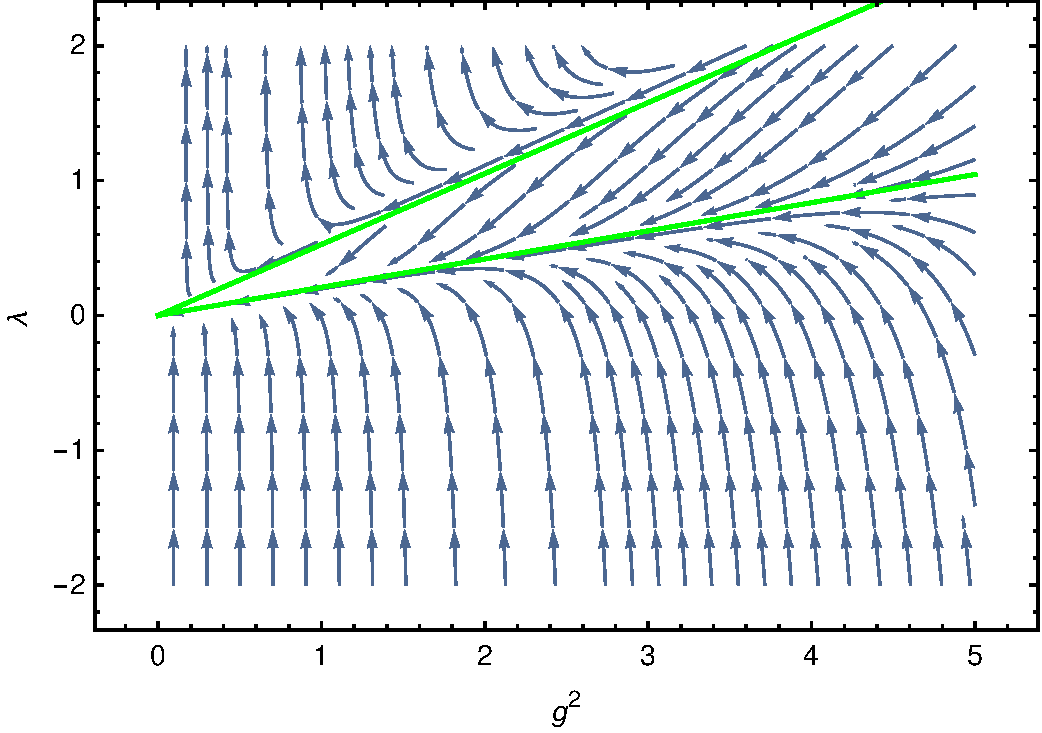
\includegraphics[width=9cm,clip]{pics/flow}
   \caption{Running of the squared gauge coupling $g^2$ and of the scalar quartic coupling $\lambda$ for a theory with SU(5) gauge group, $N_f=26$ fundamental fermions and $N_S =1$ fundamental scalars. The arrows indicate the direction of increasing energy. The green lines represent the fixed flow solutions of the renormalisation group equations, characterised by a constant ratio $\lambda/g^2$.}
  \label{flow_2D}
\end{figure}

\begin{table}[thb]
  \small
  \centering
  \caption{For different values of N, ranges in $N_f$ such that there exist completely asymptotically free solutions, in a theory with SU(N) gauge group, $N_f$ fundamental fermions and $N_S=1$ fundamental scalars.}
  \begin{tabular}{lll}\toprule
  $N$ & $N_f$  \\\midrule
  2 & No solutions \\
  3 & $15.93 < N_f < 16.25$ \\ 
  4 & 1$9.8 < N_f < 21.75$ \\
  5 & $23.56 < N_f < 27.25$ \\
  6 & $27.27 < N_f  < 32.75$ \\
  7 & $30.94 < N_f  < 38.25$ \\
  8 & $34.6 < N_f  < 43.75$ \\
  9 & $38.24 < N_f < 49.25$ \\
  10 & $41.88 < N_f < 54.75$ \\\bottomrule
  \end{tabular}
  \label{asympt_freedom}
\end{table}

\begin{figure}[thb] 
  \centering
  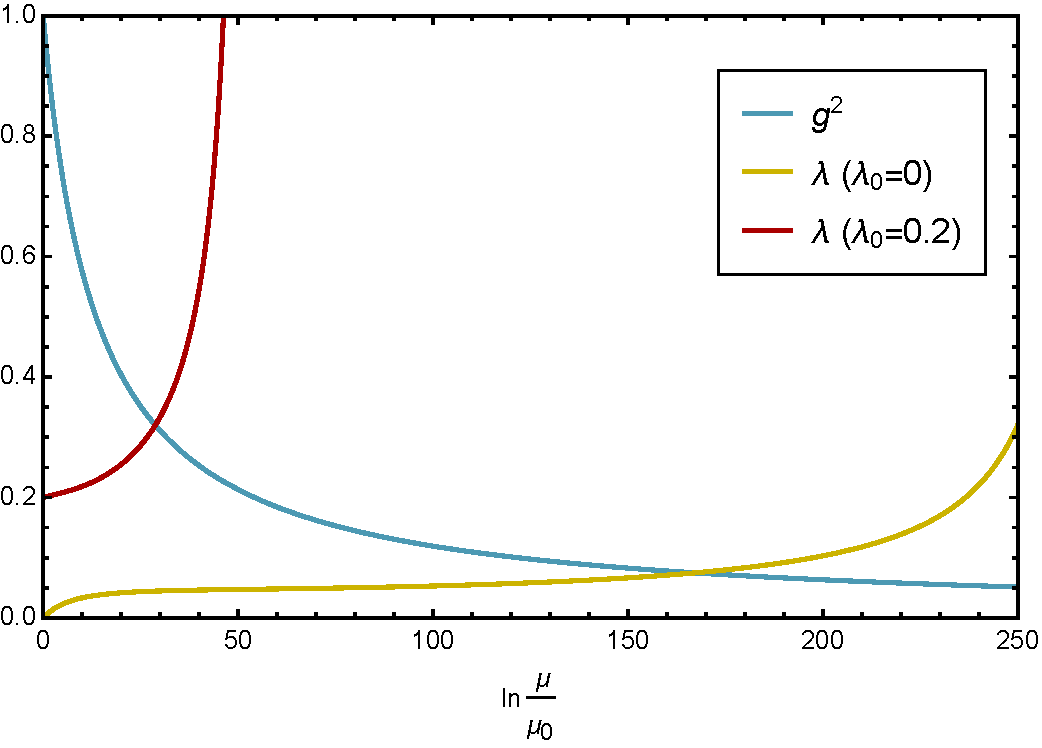
\includegraphics[width=9cm,clip]{pics/flow_N2}
  \caption{ Running of $g^2$ and $\lambda$ as functions of $\ln (\mu/\mu_0)$ in an SU(2) gauge theory with $N_f=2$ fundamental fermions and $N_S=1$ fundamental scalars. $\lambda$ is plotted for two different initial conditions: $\lambda_0 = \lambda(\mu_0) = 0$, and $\lambda_0=\lambda(\mu_0)=0.2$.}
  \label{flow_SU2}
\end{figure}

One more comment must be made regarding the case $N=2$. As previously pointed out, the fundamental representation of SU(2) is pseudo-real. One may wonder whether in this case there exist more quartic operators than the ones listed in equation \ref{quartic_operators}. It is shown in appendix \ref{app_quartic_potential} that, also in the case of an SU(2) gauge group, the most general quartic potential takes the form \ref{quartic_potential}.

%%%%%%%%%%%%%%%%%%%%%%%%%%%%%%%%%%%%%%%%%%%%%%%%%%%%%%

\section{Lattice setup}


We now move to the lattice study of the SU(2) gauge theory with two fundamental fermions and one fundamental scalar. In section \ref{running_lambda}, we discussed the running of the scalar quartic coupling, and we concluded that the SU(2) theory is not well defined at high energies because the quartic coupling diverges. Because of this, it is impossible to define the continuum limit of the lattice theory. In fact, due to the universality of the first two coefficients of the beta function, the running of the lattice bare couplings as functions of the lattice spacing is the same as shown in figure \ref{flow_SU2}, with $\mu \propto 1/a$. It follows that, at least in the region where perturbation theory is valid, there is no critical point in the space of bare lattice parameters, and the program of taking the lattice spacing to zero while moving on lines of constant physics cannot be undertaken. Instead, one can take the lattice spacing down to some small but finite value, and match the lattice theory to an effective theory with an ultraviolet cutoff. Given the running of the scalar quartic coupling shown in figure \ref{flow_SU2}, we expect the lattice theory to present a good scaling window when changing the lattice spacing, so that valuable input for phenomenological models can be provided.

For our lattice study, we generated gauge and scalar field configurations with the HiRep code, first introduced in \cite{DelDebbio:2008zf}, which we extended in order to simulate the scalar field in addition to gauge and fermions. In the following we describe the lattice action and the resulting forces needed for the implementation of the Hybrid Monte Carlo algorithm.


\subsection{Action}

For the gauge and fermion action we use the Wilson discretisation, as defined in equation \ref{lattice_action_psf}. For simplicity, we fix the lattice spacing to one, and we use the standard notation $\beta = 2 N/ g^2 = 4/g^2$. As for the scalar field $S$, we consider the Euclidean continuum action:

\begin{equation}
S_S^{cont} [A,S^{\dagger},S]= \int d^4x \biggl( (D_{\mu} S)^{\dagger} D_{\mu}S + m_S^2 |S|^ 2 + \lambda |S|^4 \biggr) \; ,
\end{equation}
%
and we discretise it by assigning 

\begin{equation}
\int \dx (D_{\mu} S)^{\dagger} D_{\mu}S \to - \sum_{x,\mu} S^{\dagger} \nabla_{\mu}^* \nabla_{\mu} S \; ,
\end{equation}
%
where

\begin{equation}
\begin{split}
&\nabla_{\mu} S(x) = U_{\mu}(x)S(x + \hat\mu) - S(x)  \\
&\nabla_{\mu}^* S(x) = S(x) - U_{\mu}(x- \hat \mu)^{\dagger} S(x- \hat \mu) \; .
\end{split}
\end{equation}
%
The resulting discretised action is: 

\begin{equation}
\begin{split}
S_S[U,S^{\dagger},S] = & \sum_x \biggl[ - \sum_{\mu} \biggl( S^{\dagger}(x) U_{\mu}(x) S(x+\hat\mu) + S^{\dagger}(x) U_{\mu}(x-\hat\mu)^{\dagger} S(x-\hat\mu) \biggr) +  \\
 & M^2 S^{\dagger}(x) S(x) + \lambda \bigl(S^{\dagger}(x) S(x) \bigr)^2 \biggr] \: ,
\end{split}
\label{scalar_lattice_action}
\end{equation}
%
where $M^2=m_S^2+8$. For future purposes, we write the action of our lattice model as:

\begin{equation}
S[U,\phi^{\dagger},\phi,S^{\dagger},S] = S_G[U] + S_F[U,\phi^{\dagger},\phi] + S_S[U,S^{\dagger},S] \: ,
\label{action}
\end{equation}
%
where $S_S$ is the scalar contribution given by equation \ref{scalar_lattice_action}, $S_G$ is the gauge contribution:

\begin{equation}
S_G[U] =  \beta \sum_{x \in \Lambda}  \sum_{\mu < \nu} \biggr[  1 - \frac{1}{\mathrm{N}} \re \tr  [U_{\mu \nu}] \biggl ] \: ,
\end{equation}
%
and $S_F$ the pseudofermion contribution:

\begin{equation}
S_F[U,\phi^{\dagger},\phi]  = \sum_{x,y \in \Lambda} \phi^{\dagger}(x) Q^{-2}(x \vert y)\phi(y) \equiv \phi^{\dagger} Q^{-2} \phi \: ,
\end{equation}
%
where we introduced a short-hand notation that will be useful in the following.


\subsection{Forces}
\label{Forces}

In order to implement the Hybrid Monte Carlo algorithm, we introduce the Hamiltonian:

\begin{equation}
H = \frac{1}{2} T_R\sum_{x,\mu}\sum_{a=1}^{N^2-1} \pi_a (x, \mu)^2 + \sum_x \sum_{i=1}^N P_i(x)P^*_i(x) + S[U,\phi^{\dagger},\phi,S^{\dagger},S] \: ,
\end{equation}
%
where $\pi_a(x,\mu)$ and $P_i(x)$ are the momenta associated to the gauge and scalar fields, and $S$ is the action \ref{action}. Here, to be more general, we are referring to an SU(N) gauge group. $T_R$ is the normalisation of the SU(N) generators in the representation $R$, defined by: $\mathrm{tr} (T^aT^b) = T_R \delta^{ab}$.
In this setup, only gauge and scalar fields evolve dynamically along the molecular dynamics trajectory. The pseudofermions are updated before starting every new trajectory according to the following rule: a field $\chi$ is extracted out of a Gaussian distribution, with probability $P[\chi] \propto \exp [-\chi^{\dagger} \chi]$, and then the pseudofermion field is defined as: $\phi = D \chi$, where $D$ is the Wilson-Dirac operator \ref{Wilson-Dirac}. The field $\phi$ defined in this way is correctly distributed according to:


\begin{equation}
\det[Q^2] = \det[D]^2 = \det[DD^{\dagger}] = \pi^{-N} \int \prod_{x \in \Lambda} \mathrm{d} \phi(x) \mathrm{d} \phi^{\dagger}(x) \exp \bigl[ 
-\phi^{\dagger}(DD^{\dagger})^{-1}  \phi \bigr] \: .
\end{equation}
%
We express the link variables as:
\begin{equation}
U_{\mu}(x)=\exp [\frac{i}{T_R} q_a(x,\mu) T^a] \: , 
\end{equation}
%
and we assign the conjugate momenta as follows:

\begin{equation}
\begin{split}
& q_a(x,\mu) \to \pi_a(x,\mu) \\
& S_i(x) \to P_i(x) \; .
\end{split}
\end{equation}
%
Hamilton's equations are given by:

\begin{equation}
\begin{split}
& \dot{q}_a(x,\mu) = \frac{\partial H}{\partial \pi_a(x,\mu)}  =T_R \pi_a(x,\mu) \\
& \dot{\pi}_a(x,\mu) = -\frac{\partial H}{\partial q_a(x,\mu)} = -\frac{\partial S_G}{\partial q_a(x,\mu)} -\frac{\partial S_F}{\partial q_a(x,\mu)} -\frac{\partial S_S}{\partial q_a(x,\mu)} \\
& \dot{S}_i(x) = \frac{\partial H}{\partial P_i(x)} = P^*_i(x) \\
& \dot{P}_i(x) =  -\frac{\partial H}{\partial S_i(x)} = -\frac{\partial S_S}{\partial S_i(x)}  \: ,\\ 
\end{split} 
\label{hamilton}
\end{equation} 
%
where the dot indicates the derivative with respect to molecular dynamics time. For brevity we omitted the equations for $\dot S^*$ and $\dot P^*$, which are simply given by the complex conjugate of the last two lines in \ref{hamilton}.
The first line of \ref{hamilton} can be rewritten in terms of the link variables as follows:


\begin{equation}
\dot{U_{\mu}}(x)= i \pi_a(x,\mu)T^a U_{\mu}(x) \; .
\end{equation}
%
The driving forces are given by:

\begin{equation}
\bullet \qquad \frac{\partial S_G}{\partial q_a(x,\mu)} = - \frac{\beta}{N} \frac{1}{T_R} \mathrm{Re \; tr} \biggl[ i T^a U_{\mu}(x) V^{\dagger}_{\mu} (x) \biggr]
\end{equation}
%
where $V_{\mu}(x) = \sum_{\nu \neq \mu} \bigl[ U_{\nu}(x) U_{\mu}(x+\hat\nu) U_{\nu}^{\dagger}(x+\hat\mu) + 
U_{\nu}^{\dagger}(x - \hat\nu) U_{\mu}(x - \hat\nu) U_{\nu}(x-\hat\nu+\hat\mu)\bigr]$ is the sum of the staples around the link $U_{\mu}(x)$,


\begin{equation}
\bullet \qquad\frac{\partial S_F}{\partial q_a(x,\mu)} =   -\biggl[ \phi^{\dagger} Q^{-2}\frac{\partial Q}{\partial q_a(x,\mu)} Q^{-1} \phi + \phi^{\dagger} Q^{-1} \frac{\partial Q}{\partial q_a(x,\mu)} Q^{-2} \phi \biggr] 
\end{equation}
%
where

\begin{equation}
\frac{\partial Q(x \vert y)}{\partial q_a(z,\mu)} = \gamma_5 \biggl( -\frac{i}{2T_R} (\id - \gamma_{\mu}) T^a U_{\mu}(z) \delta_{y,z+\hat\mu} \delta_{x,z} +\frac{i}{2T_R}(\id + \gamma_{\mu}) U_{\mu}^{\dagger}(z) T^a \delta_{y,z} \delta_{x-a\hat\mu,z} \biggr) \: ,
\end{equation}


\begin{equation}
\bullet \qquad
\frac{\partial S_S}{\partial q_a(x,\mu)} = - \frac{2}{T_R} \; \mathrm{Re} \biggl[ S^{\dagger}(x) i T^a U_{\mu}(x) S(x+\hat\mu) \biggr] 
\end{equation}



\begin{equation}
\begin{split}
\bullet \qquad
\frac{\partial S_S}{\partial S_i(x)} = & - \sum_{\mu} \biggl( S^*_k(x-\hat \mu) U_{\mu}(x-\hat\mu)_{ki} + S^*_k(x+\hat\mu) U_{\mu}(x)^{\dagger}_{ki} \biggr) +  \\
& + M^2 S_i^*(x) + 2 \lambda S_k^*(x) S_k(x) S_i^*(x) \: .
\end{split}
\end{equation}
%
Hamilton's equations \ref{hamilton} are to be solved numerically, thus generating the molecular dynamics trajectory. In this work we used a second-order Omelyan integrator \cite{PhysRevE.65.056706,OMELYAN2003272} for the numerical integration.


%%%%%%%%%%%%%%%%%%%%%%%%%%%%%%%%%%%%%%%%%%%%%%%%%%%%%%


\section{Spectrum}

\subsection{Mesons}

Finite volume corrections + dependence on $m_{PCAC}$

\subsection{Scalar-scalar states}

\subsection{Fermion-scalar states}

%%%%%%%%%%%%%%%%%%%%%%%%%%%%%%%%%%%%%%%%%%%%%%%%%%%%%%


\section{Phase space}

\subsection{Phase diagram of the SU(2)-Higgs model}

\subsection{Gauge fixing}

\subsection{Results}

%%%%%%%%%%%%%%%%%%%%%%%%%%%%%%%%%%%%%%%%%%%%%%%%%%%%%%

\section{Conclusions and outlook}

%Renormalisation, continuum limit

%%%%%%%%%%%%%%%%%%%%%%%%%%%%%%%%%%%%%%%%%%%%%%%%%%%%%%

\chapter{Transport coefficients in the conformal window}

Gauge theories with a nontrivial infrared (IR) fixed point are important in the context of model building Beyond the Standard Model \cite{Sannino:2008ha}. These theories are characterised by scale invariance in the infrared and, in the case of four space-time dimensions, they are invariant under the larger group of conformal transformations. For this reason, the region in theory space, parametrised by the number of colours ($N$) and fermion flavours ($N_f$), such that a nontrivial IR fixed point exists, is called conformal window.
Substantial effort has been taken in studying the properties of theories in the conformal window, both perturbatively and via lattice simulations (\emph{references?}). In this chapter, we present a study of the transport coefficients of theories in the perturbative conformal window, which has been published in \cite{Toniato:2016twr}.
The chapter is organised as follows: we start by introducing the conformal window and the definition of the transport coefficients under analysis. We then briefly sketch the method used by the authors of \cite{Arnold:2000dr} for calculating the transport coefficients of a gauge theory coupled to fermions. Finally, we present the results obtained by applying the perturbative results of \cite{Arnold:2000dr} to theories in the conformal window. 

%%%%%%%%%%%%%%%%%%%%%%%%%%%%%%%%%%%%%%%%%%%%%%%%%%%%%%

\section{The conformal window}
\label{ conformal_window}

We consider a non-Abelian gauge theory, with gauge group SU($N$) and $N_f$ fermions in the representation $r$. The two-loop beta function for the gauge coupling $g$ is given by:

 \begin{equation}
 \beta (g) = - \frac{\beta_0}{(4\pi)^2} g^3 - \frac{\beta_1}{(4\pi)^4} g^5 + \mathcal{O}(g^{7}) \; ,
 \label{beta_f}
 \end{equation}
%
with

 \begin{align}
\beta_0 &= \frac{11}{3} C_2[G] - \frac{4}{3} T[r] N_f\; , \\
\beta_1 &= \frac{34}{3} C_2^2[G] - \left ( \frac{20}{3} C_2[G] + 4 C_2[r] \right ) T[r] N_f\; ,
\end{align}
%
where $G$ denotes the adjoint representation. The definition of the group factors $C_2$, $T$ and $d$ can be found in appendix \ref{SUN_generators}. If $\beta_0 > 0$, the theory is asymptotically free, i.e. $g=0$ is an ultraviolet(UV)-stable fixed point of the renormalisation group (RG) flow. This happens provided the number of fermions is smaller than the upper limit:

\begin{equation}
N_f^{AF} = \frac{11}{4} \frac{C_2[G]}{T[r]} \: .
\end{equation}
%
The number of flavours and colours can be chosen such that $\beta_0>0$ and $\beta_1<0$. In this case there exists an additional zero of the beta function:

\begin{equation}
g^* = -(4 \pi)^2 \frac{\beta_0}{\beta_1} \: .
\end{equation}
%
This is an IR-stable fixed point, which can be studied in perturbation theory in case $g^*$ is small \cite{Banks:1981nn}. In particular, $g^*$ goes to zero in the limit $N_f \to N_f^{AF}$. If $g^*$ is small, the theory remains perturbative along the whole RG flow, from the UV, where it is dominated by the asymptotically free fixed point $g=0$, down to the IR. If $g^*$ is not small enough, then one has to consider higher-order terms in the beta function \ref{beta_f}, and eventually, when $g^*$ leaves the perturbative regime, apply non-perturbative methods such as lattice simulations. In theory space, parametrised by $N$ and $N_f$, the upper boundary of the conformal window for every fixed $N$ is given by $N_f = N_f^{AF}$, while the lower boundary is yet to be found via non-perturbative methods, since the value of $g^*$ increases with decreasing $N_f$.


\begin{figure}[h!]
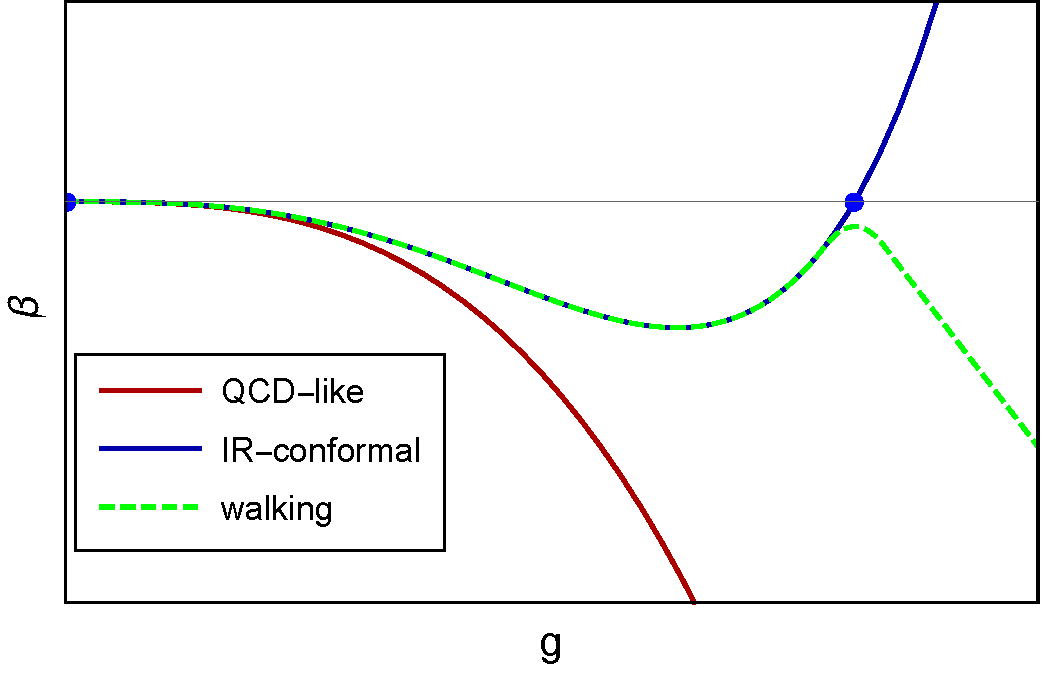
\includegraphics[width=0.5\textwidth]{pics/beta_walking}~~~
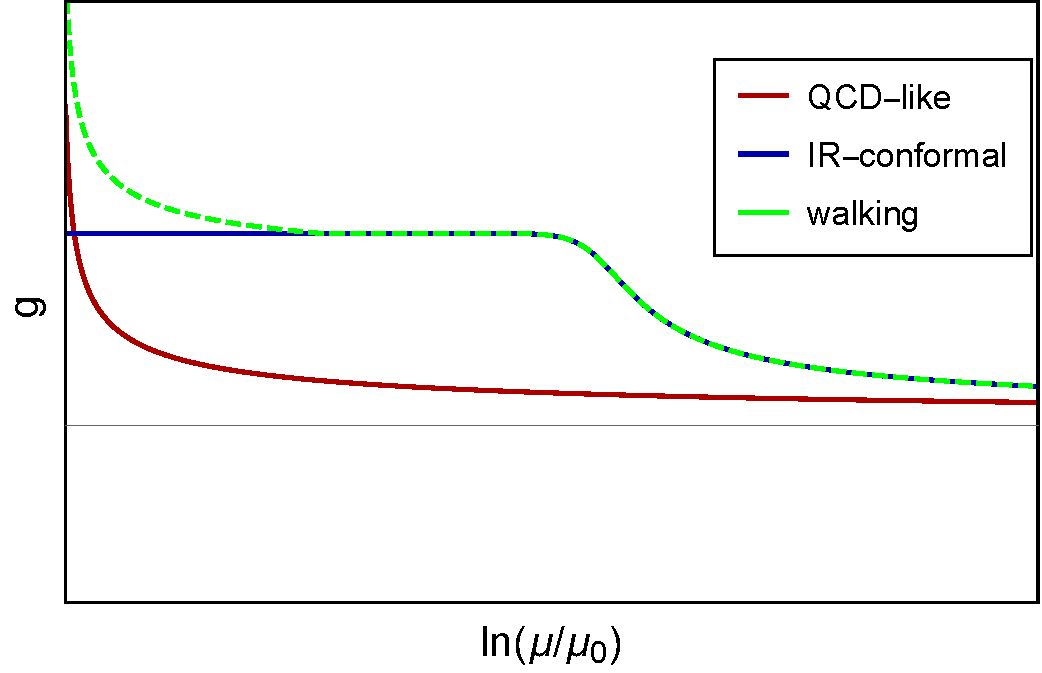
\includegraphics[width=0.5\textwidth]{pics/g_walking}
\caption{Beta function (left panel) and gauge coupling (right panel) for three different kinds of theories: a QCD-like theory (red line), a theory in the conformal window (blue line) and a theory with walking gauge coupling (green dashed line). In the right panel, the gauge coupling is plotted as a function of the energy scale $\mu$ over some reference scale $\mu_0$.} 
\label{walking}
\end{figure}


Figure \ref{walking} shows three different regimes of the beta function, and the related running of the gauge coupling. The first one (red line) characterises a QCD-like theory. The beta function has one single zero at $g=0$, and is negative for all other values of $g$. In this case, the coupling goes to zero in the UV (asymptotic freedom) and grows when moving towards the IR, until it diverges at some finite energy scale. This theory displays spontaneous chiral symmetry breaking in the IR. The second regime (blue line) characterises a theory in the conformal window. The beta function has two zeros, $g=0$ and $g=g^*$, and is negative in between. The gauge coupling goes to zero in the UV, and stabilises at the fixed point value $g=g^*$ in the IR. This theory is characterised by scale invariance in the IR, and does not display spontaneous chiral symmetry breaking. The third regime (green dashed line) is associated to "walking" dynamics. It is reasonable to assume that, close to the lower boundary of the conformal window, theories with an approximate IR fixed point can be found. Their beta function is very similar to the one of theories in the conformal window, with the difference that it gets very close to zero at $g\simeq g^*$, without actually reaching a fixed point, and then assumes a QCD-like behaviour for larger values of $g$. In this theory the gauge coupling goes to zero in the UV, then stabilises at an approximately constant value for a wide range of energies, and finally diverges at a finite energy scale, thus triggering chiral symmetry breaking. Theories with walking gauge coupling are very important in the context of composite Higgs models, as discussed in section \ref{partial_comp}. In fact these theories show an approximate conformal behaviour, which can lead to a nice separation of scales and good scaling properties of composite operators, and at the same time break chiral symmetry, which is a necessary ingredient in composite Higgs models.
Lattice simulations can be used in order to find out whether a theory is in one of the three regimes shown in figure \ref{walking}, see for example \cite{Hietanen:2008mr,Hansen:2017ejh}.

Here we consider theories in the perturbative conformal window, i.e. $N_f \lesssim N_f^{AF}$, and we study their sheer viscosity and fermion number diffusion coefficient by applying the perturbative results obtained in \cite{Arnold:2000dr}.

%REMEMBER TO JUSTIFY THE FACT THAT THE NUMBER OF FLAVOURS IS TREATED LIKE A CONTINUOUS PARAMETER!

%%%%%%%%%%%%%%%%%%%%%%%%%%%%%%%%%%%%%%%%%%%%%%%%%%%%%%

\section{Transport coefficients}

Transport coefficients characterise the response of a fluid to small deviations from thermodynamic equilibrium. The transport coefficients considered in our study are viscosity and diffusion coefficients. Viscosity describes the response to spacial variations of the flow velocity, in the presence of dissipative phenomena (internal friction). Diffusion coefficients describe the evolution of the density of conserved charges, when the charge concentration is not uniform over the fluid. In this section we introduce the equations of motion of a viscous fluid and the diffusion equation, which provide the definitions of the transport coefficients under analysis.

\subsection{Viscosity}

In this derivation we follow the lines of \cite{landau2013fluid}. We start by considering the motion of an ideal fluid, which is described by the continuity equation:

\begin{equation}
\partial_t \rho + \partial_i (\rho v_i) = 0 \: ,
\end{equation}
%
and Euler's equation (given here in component form):

\begin{equation}
\partial_t v_i +  v_j \partial_j v_i = -\frac{1}{\rho} \partial_i p \: ,
\end{equation}
%
where time is denoted by $t$, spacial coordinates by $x_i$ ($i=1,2,3$), the fluid mass density by $\rho$, the flow velocity components by $v_i$,  and the pressure by $p$. Sums over repeated indices are understood. Euler's equation can be rewritten as:

\begin{equation}
\partial_t (\rho v_i) = - \partial_j \Pi_{ij} \: ,
\label{Euler}
\end{equation}
%
where the symmetric tensor $\Pi_{ij} = p \delta_{ij} + \rho v_i v_j$ represents the flux density of the momentum component $i$ in all possible directions $j$. The momentum transfer described by the tensor $\Pi_{ij}$ is reversible, and it is due to the mechanical transport of the different volumes of fluid and to pressure forces acting in the fluid. The motion of a viscous fluid is characterised by an extra, irreversible, transfer of momentum, occurring from points where the flow velocity is large to points where is is low.
In the case of a viscous fluid, the tensor $\Pi_{ij}$ can be parametrised as:

\begin{equation}
\Pi_{ij} = p \delta_{ij} + \rho v_i v_j - \sigma_{ik} \: ,
\end{equation}
%
where $-\sigma_{ik}$ is the contribution due to internal friction. Always following \cite{landau2013fluid}, we notice that $\sigma_{ik}$ must depend on the spacial derivatives of the flow velocity, since internal friction occurs only when different layers of fluid move with different velocities, and must vanish when the flow velocity is constant in space. Moreover, $\sigma_{ij}$
must vanish when the fluid is in uniform rotational motion, because in this case there is no relative motion between different layers of fluid. The flow velocity of a uniformly rotating fluid is expressed as: $\vec v = \vec \Omega \times \vec r$, $\vec r$ being the distance from the centre of rotation and $\vec \Omega$ the constant angular velocity. If the velocity gradients are small, we may assume that $\sigma_{ik}$ is a linear function of the first derivatives of the flow velocity. The most general function of this sort, which vanishes in case of constant $\vec v$, or $\vec v = \vec \Omega \times \vec r$, is:

\begin{equation}
\sigma_{ij} = \eta \biggl( \partial_i v_j + \partial_j v_i -\frac{2}{3} \delta_{ij} \partial_k v_k \biggr) + \zeta \delta_{ij} \partial_{k} v_k \: ,
\label{viscosity_classical}
\end{equation}
%
where the coefficient $\eta$ is the shear viscosity and $\zeta$ the bulk viscosity. The terms in equation \ref{viscosity_classical} are organised so that the expression in parentheses vanishes when tracing over $i$ and $j$. To conclude, we have for a viscous fluid:

\begin{equation}
\Pi_{ij} = p \delta_{ij} + \rho v_i v_j - \eta \biggl( \partial_i v_j + \partial_j v_i -\frac{2}{3} \delta_{ij} \partial_k v_k \biggr) - \zeta \delta_{ij} \partial_{k} v_k \: ,
\label{Navier-Stokes}
\end{equation}
%
and Euler's equation is substituted by the Navier-Stokes equation, obtained by inserting \ref{Navier-Stokes} in \ref{Euler}.


A fluid with relativistic flow velocity, or having microscopic components moving at relativistic speed, is described by relativistic fluid equations.
 
 \subsection{Diffusion coefficient}


%%%%%%%%%%%%%%%%%%%%%%%%%%%%%%%%%%%%%%%%%%%%%%%%%%%%%%

\section{Transport coefficients of a gauge theory: kinetic approach}

The equilibrium state of a high temperature quantum field theory can be described as a relativistic fluid. Transport coefficients can in principle be computed, based on the dynamics of the underlying microscopic theory.
This is what the authors of \cite{Arnold:2000dr,Arnold:2003zc} did in the case of a weakly coupled , high temperature gauge theory, both in a leading-log approximation \cite{Arnold:2000dr} and in a full leading order treatment \cite{Arnold:2003zc}.
In this section, without aiming at a complete description, we would like to sketch the method used in these works to compute the transport coefficients. The analytic results given in \cite{Arnold:2000dr}, together with the coefficients in table \ref{AB}, are the basis for our study of transport coefficients in the perturbative conformal window.

In \cite{Arnold:2000dr,Arnold:2003zc}, a finite-temperature gauge theory coupled to fermions is considered, under the assumption that the gauge coupling at the scale of the temperature is weak: $g(T) \ll 1$.

\subsection{Leading-log and next-to-leading-log results}

    \begin{table}[h!]
\begin{center}
    %\begin{minipage}{3.8in}
    \begin{tabular}{c||ccc }
    $N_f$ & $ \quad A$ & $\quad B $ &   \\
    \hline \hline
    $ 6 $ & \quad 2.918 & \quad 3.064   \\
        $14$ &\quad 2.878 &\quad 3.135  \\
        $15$ & \quad 2.873 & \quad 3.172 \\
        $16$ & \quad 2.869  & \quad 3.176 \\
    $16.25$ & \quad 2.867 & \quad 3.177
    \end{tabular}
    %\end{minipage}
    \end{center}
\caption{Values of the coefficients $A$ and $B$ \cite{privcommGDM}
appearing in the next-to-leading-log expressions of the shear viscosity and the fermion-number diffusion coefficient, 
for $N = 3$ and different values of $N_f$.}
\label{AB}
    \end{table}


%%%%%%%%%%%%%%%%%%%%%%%%%%%%%%%%%%%%%%%%%%%%%%%%%%%%%%

\section{Application to theories in the conformal window}

%%%%%%%%%%%%%%%%%%%%%%%%%%%%%%%%%%%%%%%%%%%%%%%%%%%%%%

\chapter{Conclusions}


In this thesis, we presented our results of two studies of non-Abelian gauge theories applied to Beyond the Standard model physics. 
The first study, based on non-perturbative lattice techniques, is part of the ongoing large effort to explore composite Higgs models. 
More specifically, our study aims at providing non-perturbative information on the dynamics of fundamental partial compositeness models, featuring fermionic and scalar matter fields.
With this motivation, we studied on the lattice the SU(2) gauge theory with two fundamental fermions and one fundamental scalar. Given the very large parameter space of this lattice theory, our analysis is still preliminary, but nevertheless it already provides some interesting results. 
We have found evidence of a phase with broken fermion flavour symmetry, which seems to confirm the existence of the scenario postulated in fundamental partial compositeness models. 
Moreover, we found a very impressive agreement between chiral extrapolations of the meson spectrum obtained in our model and in the SU(2) lattice theory with two fundamental fermions and no scalar. 
We also addressed the question of gauge symmetry breaking induced by the scalar field, and discussed whether regions of broken and unbroken symmetry can be uniquely identified in the phase diagram. We found evidence of a symmetry-breaking transition accompanied by a thermodynamic transition affecting all the considered observables.

In the second study, we presented a perturbative computation of the transport coefficients for theories in the conformal window. 
This class of theories is very relevant in the context of Beyond the Standard Model physics, in particular for composite Higgs models. We applied perturbative results for the transport coefficients of a hot gauge theory to theories with an infrared perturbative fixed point. One interesting point of our analysis is that it provides a framework in which the perturbative results hold both at high and low temperatures, due to the perturbative nature of the infrared fixed point. 
However, it turns out that the results are quantitatively (and even just qualitatively) trustable in a very restricted range of the conformal window. 
\appendix

\chapter{}

\section{General conventions and definitions}

In this appendix we introduce the general notations and conventions used in the thesis. 

\subsection{Metric and units}

We use the following convention for Minkowski metric:

\begin{equation}
(\eta_{\mu\nu}) = \mathrm{diag}[1,-1,-1,-1] \: .
\label{metric}
\end{equation}

As for the unit system, we use natural units, where both the speed of light $c$ and the reduced Planck constant $\hbar$ are set equal to one.

\subsection{Gamma matrices}
\label{gamma_matrices}

Gamma matrices appear in the Dirac Lagrangian: $\Lag_D [\bar \psi, \psi] = \bar \psi (i \gamma^{\mu} D_{\mu} -m \id) \psi$, and fulfil the following relations:

\begin{itemize}
\item Clifford algebra: $\qty \big{\gamma^{\mu}, \gamma^{\nu}} = 2 \id \eta^{\mu \nu}$
\item Relation with the hermitian conjugate: $\gamma^{\mu} = \gamma^0 (\gamma^{\mu})^{\dagger} \gamma^0$ \: .
\end{itemize}
%
As a consequence, the following equations hold:
\begin{itemize}
\item $(\gamma^0)^2 = \id$, $(\gamma^i)^2 = - \id$, $i= 1,2,3$
\item $(\gamma^0)^{\dagger} = \gamma^0$, $(\gamma^i)^{\dagger} = -\gamma^i$, $i= 1,2,3$
\item $\qty \big{\gamma^{\mu}, \gamma^{\nu}} = 0$ if $\mu \neq \nu$ \: .
\end{itemize}

$\gamma_5$ is defined by: $\gamma_5 = i \gamma^0 \gamma^1 \gamma^2 \gamma^3$, and it has the following properties: $(\gamma_5)^2=\id$, $(\gamma_5)^{\dagger} = \gamma_5$, $\qty \big{\gamma_5, \gamma^{\mu}} = 0$. There exist multiple representations of the gamma matrices, and physical results do not depend on the choice of the representation. In this thesis we use the chiral representation:

\begin{equation}
\gamma^0 = 
\begin{pmatrix}
0 & \id_{2 \times 2} \\
\id_{2 \times 2} & 0
\end{pmatrix}
\: ,
\qquad
\gamma^i = 
\begin{pmatrix}
0 & \sigma^i \\
-\sigma^i & 0
\end{pmatrix}
\: ,
\qquad
\gamma_5 = 
\begin{pmatrix}
-\id_{2 \times 2} & 0 \\
0  & \id_{2 \times 2}
\end{pmatrix}
\: ,
\end{equation}
%
where $\sigma^i$, $i=1,2,3$, are the Pauli matrices.

Gamma matrices are involved in the definition of the Lorentz group representation acting on Dirac spinors. In particular, the generators of Lorentz transformations are defined by: $J^{\mu \nu} = -i/4 [\gamma^{\mu},\gamma^{\nu}]$. Moreover, the parity transformation of a Dirac spinor is defined by:

\begin{equation}
\psi(\textbf x, t) \to \psi'(\textbf x, t) = \gamma^0 \psi(-\textbf x, t) \: ,
\end{equation}
%
and the transformation under charge conjugation by:

\begin{equation}
\psi(x) \to \psi^C(x) = C \bar \psi(x)^T \: ,
\end{equation}
%
where the charge conjugation operator is $C = i \gamma^2 \gamma^0$.

$\gamma_5$ appears in the definition of the chirality projectors:

\begin{equation}
P_L = \frac{\id - \gamma_5}{2} \: , \qquad P_R = \frac{\id + \gamma_5}{2} \: ,
\end{equation}
%
which have the following properties: $P_{R,L}^2 = P_{R,L}$, $P_R P_L = P_L P_R = 0$, $P_L + P_R = \id$, and are used to define left- and right-handed spinors:

\begin{equation}
\psi(x) = \psi_L(x)+ \psi_R(x) \: , \qquad\psi_L(x) = P_L \psi(x) \: , \qquad \psi_R(x) = P_R \psi(x) \: .
\end{equation}
%
The Dirac Lagrangian can be rewritten in terms of left- and right-handed Dirac spinors as follows:

\begin{equation}
\Lag_D = \bar \psi_L (i \gamma^{\mu} D_{\mu}) \psi_L + \bar \psi_R (i \gamma^{\mu} D_{\mu}) \psi_R -m (\bar\psi_L \psi_R + \bar\psi_R \psi_L) \: .
\end{equation}

The Dirac Lagrangian in Euclidean space is: $\Lag_D^E [\bar \psi, \psi] = \bar \psi (\gamma_{\mu}^E D_{\mu} + m \id) \psi$, where the relation between Minkowskian and Euclidean gamma matrices is:

\begin{equation}
\gamma_0^E = \gamma_0 \: , \qquad \gamma_i^E = i \gamma_i = -i \gamma^i \: .
\end{equation}
%
Euclidean gamma matrices have the following properties: 

\begin{itemize}
\item $\qty \big{\gamma_{\mu}^E, \gamma_{\nu}^E} = 2 \id \delta_{\mu \nu} \Rightarrow (\gamma_{\mu}^E)^2 = \id$
\item $(\gamma_{\mu}^E)^{\dagger} = \gamma_{\mu}^E$
\end{itemize}

Euclidean $\gamma_5$ is defined by: $\gamma_5^E =  \gamma_1^E \gamma_2^E \gamma_3^E \gamma_0^E$, and has analogue properties to Minkowskian $\gamma_5$: $(\gamma_5^E)^2=\id$, $(\gamma_5^E)^{\dagger} = \gamma_5^E$, $\qty \big{\gamma_5^E, \gamma_{\mu}^E} = 0$.

Euclidean gamma matrices in the chiral representation are given by:

\begin{equation}
\gamma_0^E = 
\begin{pmatrix}
0 & \id_{2 \times 2} \\
\id_{2 \times 2} & 0
\end{pmatrix}
\: ,
\qquad
\gamma_i^E = 
\begin{pmatrix}
0 & -i \sigma^i \\
i \sigma^i & 0
\end{pmatrix}
\: ,
\qquad
\gamma_5^E = 
\begin{pmatrix}
\id_{2 \times 2} & 0 \\
0  & -\id_{2 \times 2}
\end{pmatrix}
\: .
\end{equation}

In this thesis we always omit the superscript $E$ in gamma matrices, and we implicitly assume that every time we discuss a lattice model, which requires the Euclidean version of the action, gamma matrices assume their Euclidean form.

\subsection{SU($N$) generators}
\label{SUN_generators}

We denote the generators of the representation $r$ of SU($N$) by $T^a_r$, with $a = 1, \dots, N^2 -1$. The generators are normalised as:

\begin{equation}
\tr [T^a_r T^b_r] = T[r] \delta^{ab} \: .
\end{equation}
%
The quadratic Casimir $C_2[r]$ is defined by:

\begin{equation}
\sum_{a=1}^{N^2 -1} T^a_r T^a_r = C_2[r] \id \: ,
\end{equation}
%
and it is related to $T[r]$ and the dimension of the representation $d[r]$ by:

\begin{equation}
C_2[r] d[r] = T[r] d[G] \: ,
\end{equation}
%
where $G$ denotes the adjoint representation. The values of $d$, $T$ and $C_2$ for the fundamental and adjoint representation are listed in table \ref{group_factors}.

    \begin{table}
\begin{center}
    %\begin{minipage}{3.8in}
    \begin{tabular}{c||ccc }
    $r$ & $ \quad T[r] $ & $\quad C_2[r] $ & $\quad d[r] $  \\
    \hline \hline
    $ \fund $ & $\quad \frac{1}{2}$ & $\quad\frac{N^2-1}{2N}$ &\quad $N$  \\
        $\text{$G$}$ &\quad $N$ &\quad $N$ &\quad $N^2-1$  \\
    \end{tabular}
    %\end{minipage}
    \end{center}
\caption{Values of $d$, $T$ and $C_2$ for the fundamental ($\fund$) and adjoint (G) representation of SU($N$).}
\label{group_factors}
    \end{table}



\section{Lattice Fourier transforms}
\label{Fourier}

In this appendix we define Fourier transforms on the lattice. The lattice $\Lambda$ is defined as: 

\begin{equation}
\Lambda = \set{x_{\mu} = n_{\mu} a  \mid  n_{\mu}  = 0, \dots, L_{\mu} -1, \; \mu = 0, \dots, 3 } \; ,
\end{equation}
%
where $a$ is the lattice spacing and $L_{ \mu}$ the number of lattice points in direction $\mu$. The total number of lattice points $V$ is given by: $V = \prod_{\mu=0}^3 L_{\mu}$.

We consider a function $f(x)$ defined on the lattice, and we define its Fourier transform as:

\begin{equation}
\begin{split}
&f(x) = \frac{1}{\sqrt V} \sum_{p \in \tilde\Lambda} \tilde f(p) e^{i p \cdot x}\\
&\tilde f(p) = \frac{1}{\sqrt V} \sum_{x \in \Lambda}  f(x) e^{-i p \cdot x}
\end{split}
\end{equation}
%
where $\tilde\Lambda$ denotes the momentum space. Since the space-time has a finite volume, the momenta belong to a discrete set. Specifically, if periodic boundary conditions are imposed in direction $\mu$, i.e. $f(x+aL_{\mu} \hat\mu) = f(x)$, then $p_{\mu}$ takes values in the discrete set $\set{p_{\mu} = \frac{2\pi}{a L_{\mu}} k_{\mu} \mid k_{\mu} \in \mathbb{Z}}$. While in the case of anti-periodic boundary conditions, $f(x+aL_{\mu} \hat\mu) = -f(x)$, $p_{\mu}$ belongs to $\set{p_{\mu} = \frac{2\pi}{a L_{\mu}} (\frac{1}{2} + k_{\mu}) \mid k_{\mu} \in \mathbb{Z}}$. Moreover, since the coordinates $x_{\mu}$ of each lattice point are represented by integer numbers of lattice spacings, the momenta are periodic: $\tilde f(p) = \tilde f(p + \frac{2\pi}{a}\hat\mu)$. Therefore, the momentum space is defined as:

\begin{equation}
\tilde\Lambda = \set{p_{\mu} = \frac{2 \pi}{a L_{\mu}}(k_{\mu} + \theta_{\mu})  \mid  k_{\mu} = -\frac{L_{\mu}}{2} + 1, \dots, \frac{L_{\mu}}{2}, \; \mu = 0, \dots, 3 } \: ,
\end{equation}
%
where $\theta_{\mu} = 0$ corresponds to periodic boundary conditions in direction $\mu$, and $\theta_{\mu} = 1/2$ to anti-periodic ones.

The lattice delta functions are defined as:

\begin{equation}
\begin{split}
& \delta(x-x') =  \delta_{n_0,n'_0} \delta_{n_1,n'_1} \delta_{n_2,n'_2} \delta_{n_3,n'_3} = \frac{1}{V} \sum_{p \in \tilde\Lambda}
e^{i p \cdot (x - x')} \\
& \delta(p-p') =  \delta_{k_0,k'_0}\delta_{k_1,k'_1} \delta_{k_2,k'_2} \delta_{k_3,k'_3} = \frac{1}{V} \sum_{x \in \Lambda} 
e^{i (p - p') \cdot x } \: .
\end{split}
\end{equation}

\section{Hybrid Monte Carlo and the detailed balance relation}
\label{HMC_db}

In this appendix we show that the HMC algorithm respects the detailed balance relation \ref{detailed_bal}. We consider a scalar field theory with action $S[\phi]$. According to equation \ref{O_HMC}, the expectation value of an observable $O$ is given by:

\begin{equation}
\langle O \rangle = \frac{\int \prod_{x} \mathrm{d} \phi(x) \mathrm{d} \pi(x) \: O[\phi] e^{-H[\pi,\phi] }}{\int \prod_{x} \mathrm{d} \phi(x) \mathrm{d} \pi(x) \: e^{-H[\pi,\phi]}} \: ,
\end{equation}
%
where the Hamiltonian is defined by: $H[\pi,\phi] =  \frac{1}{2} \sum_x \pi(x)^2 + S[\phi]$.

 The HMC algorithm consists of the following steps:

\begin{itemize}
\item The momenta $\pi(x)$ are extracted from a Gaussian distribution, with probability $P[\pi(x)] \propto \exp[-\pi(x)^2/2]$. This way an initial configuration of the momenta is defined
\item Starting from the initial configuration $(\pi, \phi)$, the system evolves to a new state $(\pi',\phi')$ along a molecular dynamics trajectory which is a numerical solution of Hamilton's equations \ref{Hamilton_eq}
\item The final configuration $(\pi',\phi')$ is accepted or rejected in a Metropolis step, according to the transition probability 
\begin{equation}
W_M(\pi, \phi \to \pi' \phi') = \min \biggl[ 1, \frac{e^{-H[\pi',\phi']}}{e^{-H[\pi,\phi]}} \biggr] \: .
\end{equation}
\end{itemize}

We denote by $W_{\mathrm{md}}(\pi,\phi \to \pi',\phi')$ the probability of evolving from the state $(\pi,\phi)$ to $(\pi',\phi')$ along the molecular dynamics trajectory.  We stress however that molecular dynamics is a deterministic process, and, given an initial state, all the following states in the trajectory are uniquely determined.

We further assume that the numerical integrator generating the molecular dynamics trajectory fulfils the following conditions:

\begin{itemize}
\item Preservation of the integration measure: $ \prod_{x} \mathrm{d} \phi(x) \mathrm{d} \pi(x) =  \prod_{x} \mathrm{d} \phi'(x) \mathrm{d} \pi'(x)$
\item Reversibility: $W_{\mathrm{md}}(\pi,\phi \to \pi',\phi') = W_{\mathrm{md}}(-\pi',\phi' \to -\pi,\phi )$\: .
\end{itemize}


The probability to evolve from a scalar field configuration $\phi$ to $\phi'$ in one HMC step is given by:

\begin{equation}
W(\phi \to \phi') = \int \prod_{x} \mathrm{d} \pi(x) \mathrm{d} \pi'(x)  W_M(\pi,\phi \to \pi',\phi') W_{\mathrm{md}}(\pi,\phi \to \pi',\phi') e^{-\sum_x \pi(x)^2 /2} \: .
\label{proof1}
\end{equation}
%
We rewrite Metropolis transition probability as follows:

\begin{equation}
\begin{split}
W_M(\pi,\phi \to \pi',\phi') & = \min \biggl[ 1, \frac{e^{-H[\pi',\phi']}}{e^{-H[\pi,\phi]}} \biggr] = 
 \frac{e^{-H[\pi',\phi']}}{e^{-H[\pi,\phi]}} \min \biggl[ 1, \frac{e^{-H[\pi,\phi]}}{e^{-H[\pi',\phi']}} \biggr]  = \\
& = \exp \biggl[ - \frac{1}{2} \sum_x \pi'(x)^2 - S[\phi'] +  \frac{1}{2} \sum_x \pi(x)^2 + S[\phi] \biggr]  W_M(\pi',\phi' \to \pi,\phi) \: ,
\end{split}
\end{equation}
%
and we insert this expression in equation \ref{proof1}:

\begin{equation}
\begin{split}
W(\phi \to \phi') = & \int \prod_{x} \mathrm{d} \pi(x) \mathrm{d} \pi'(x) W_M(\pi',\phi' \to \pi,\phi)  W_{\mathrm{md}}(\pi,\phi \to \pi',\phi') \times \\
&  \exp \biggl[- \frac{1}{2} \sum_x \pi'(x)^2 - S[\phi'] + S[\phi] \biggr]  \:  .  
\end{split}
\end{equation}

We now use the  reversibility of the molecular dynamics trajectory, together with the fact that $W_M(\pi,\phi \to \pi',\phi')$ is quadratic in $\pi$ and $\pi'$:

\begin{equation}
\begin{split}
W(\phi \to \phi') = & \exp \bigl[ - S[\phi'] + S[\phi] \bigr] \int \prod_{x} \mathrm{d} \pi(x) \mathrm{d} \pi'(x) W_M(-\pi',\phi' \to -\pi,\phi) \times \\
& W_{\mathrm{md}}(-\pi',\phi' \to -\pi,\phi) \exp \bigl[ -\sum_x \pi'(x)^2 /2 \bigr] = \\
= &  \exp \bigl[ - S[\phi'] + S[\phi] \bigr] W(\phi' \to \phi) \: ,
\end{split}
\label{proof2}
\end{equation}
%
where in the last step we used the fact that the integration measure $ \int \prod_{x} \mathrm{d} \pi(x) \mathrm{d} \pi'(x)$ and the factor $\exp \bigl[ -\sum_x \pi'(x)^2 /2 \bigr]$ are invariant under a change of sign of $\pi$ and $\pi'$. The detailed balance relation follows directly from equation \ref{proof2}:

\begin{equation}
\exp \bigl[ -  S[\phi] \bigr]W(\phi \to \phi') =\exp \bigl[ - S[\phi'] \bigr] W(\phi' \to \phi) \: .
\end{equation}

In the above proof we used explicitly the reversibility of the molecular dynamics process. The preservation of the integration measure $ \prod_{x} \mathrm{d} \phi(x) \mathrm{d} \pi(x) =  \prod_{x} \mathrm{d} \phi'(x) \mathrm{d} \pi'(x)$ is also required, because it ensures that in the path integral  $\int \prod_{x} \mathrm{d} \phi(x) \mathrm{d} \pi(x) \: e^{-H[\pi,\phi]}$ each configuration is actually weighted by $e^{-H[\pi,\phi]}$, without the appearance of an extra Jacobian determinant. (????????????????????????????)


\section{Scalar quartic potential in an SU(2) gauge theory}
\label{app_quartic_potential}

We consider a theory of gauge-interacting scalars in the fundamental representation of the gauge group SU(2). We discuss which terms are allowed by colour and flavour symmetries in the quartic potential.

\subsection{Single scalar field}


We first consider the case of one single scalar field $\phi$. A gauge transformation is given by:
%
\begin{equation}
\phi \to \phi' = U \phi
\end{equation}
%
where $U \in$ SU(2)=Sp(2) is characterised by: 
%
\begin{equation}
\begin{cases}
U^{\dagger}U = \id \\
U^{T}\epsilon U = \epsilon
\end{cases} \: ,
\end{equation}
%
$\epsilon$ being the two-dimensional antisymmetric tensor:
%
\begin{equation}
\epsilon =
\begin{pmatrix}
0 & 1 \\
-1 & 0
\end{pmatrix} \, .
\end{equation}
%
We can construct a field $\tilde{\phi}=-\epsilon \phi^*$ which transforms in the same way as $\phi$ under a gauge transformation:  $\tilde{\phi} \to \tilde{\phi}' = U \tilde{\phi}$.
%
We define a matrix $S$

\begin{equation}
S = (\phi, \tilde{\phi})
\label{S1}
\end{equation}
%
which transforms as: $S \to S'= US$.
The relation $\tilde{\phi}=-\epsilon \phi^*$ is translated in a relation between $S$ and $S^*$:

\begin{equation}
S^* = - \epsilon S E \, ,
\label{constraint}
\end{equation}
%
where
%
\begin{equation}
E =
\begin{pmatrix}
0 & 1 \\
-1 & 0
\end{pmatrix} \, .
\end{equation}
%
Eq.~\ref{constraint} can be verified as follows: we write the entries of $S$ as $S_{ia}$, where $i = 1,2$ is the colour index and $a = 1,2$ is the flavour index, then we have $S_{i1} = \phi_i$, $S_{i2} = - \epsilon_{ij} \phi^*_j = - \epsilon_{ij} S^*_{j1}$. It follows that:

\begin{equation}
\begin{split}
& (\epsilon S E)_{i1} = \epsilon_{ij} S_{ja} E_{a1} = - \epsilon_{ij} S_{j2} = -\epsilon_{ij} (- \epsilon_{jk} S_{k1}^*) = -\delta_{ik}S_{k1}^* = -S_{i1}^* \\
& (\epsilon S E)_{i2} = \epsilon_{ij} S_{ja} E_{a2} = \epsilon_{ij} S_{j1} = - S_{i2}^*
\end{split} \: .
\end{equation}
%
The kinetic term of the scalar Lagrangian is expressed in terms of $S$ as follows:

\begin{equation}
\mathcal{L}_{kin} = \frac{1}{2} \mathrm{Tr} \bigl[ (D_{\mu}S)^{\dagger} (D^{\mu}S) \bigr] \, .
\label{kin}
\end{equation}
%
Given a matrix $M \in$ U(2) we define a flavour transformation

\begin{equation}
S \to S' = SM \: ,
\end{equation}
%
and we work out the conditions under which it is a symmetry of the kinetic term \ref{kin}. If we require $S'^* = - \epsilon S' E$, it follows that $M$ must fulfil the following constraint:

\begin{equation}
EM^* = ME \: ,
\end{equation}
%
which, together with the fact that M is a unitary matrix, implies:

\begin{equation}
E=MEM^T \, .
\end{equation}
%
The flavour symmetry group is therefore Sp(2)=SU(2).

The possible terms which are quartic in the field $\phi$ and symmetric under colour and flavour transformations are the following:

\begin{equation}
\begin{split}
& \bigl( \mathrm{Tr} \bigl[ S^{\dagger} S \bigr] \bigr)^2 \\
& \mathrm{Tr} \bigl[ S^{\dagger} S S^{\dagger} S\bigr] \\
&  \bigl( \mathrm{Tr} \bigl[ S^T \epsilon S E \bigr] \bigr)^2 \\
& \mathrm{Tr} \bigl[ S^T \epsilon S E S^T \epsilon S E\bigr] \\
\end{split} \: .
\label{quartic}
\end{equation}
%
The last two terms in \ref{quartic} can be shown to be equal to the first ones by applying equation \ref{constraint}:

\begin{equation}
\begin{split}
\bigl( \mathrm{Tr} \bigl[ S^T \epsilon S E \bigr] \bigr)^2  &=   \bigl( \mathrm{Tr} \bigl[ S^T (-S^*) \bigr] \bigr)^2 =  \bigl( - \mathrm{Tr} \bigl[ (S^{\dagger} S)^* \bigr] \bigr)^2 \\
 & = \bigl(  \mathrm{Tr} \bigl[ (S^{\dagger} S) \bigr] \bigr)^2 
 \end{split} \: ,
 \label{proof1}
\end{equation}

\begin{equation}
\begin{split}
\mathrm{Tr} \bigl[ S^T \epsilon S E S^T \epsilon S E\bigr]  & = \mathrm{Tr} \bigl[ S^T (-S^*) S^T (-S^*) \bigr] = \mathrm{Tr} \bigl[ (S^{\dagger} S)^* (S^{\dagger} S)^*) \bigr] \\
& =\mathrm{Tr} \bigl[ S^{\dagger} S S^{\dagger} S\bigr] \, .
\end{split}
\label{proof2}
\end{equation}
%
The first and the second term in equation \ref{quartic} are not linearly independent when only one scalar field is present. To show this we start by explicitly writing $S^{\dagger} S$:

\begin{equation}
\begin{split}
& S^{\dagger} S = 
\begin{pmatrix}
\phi^{\dagger}\phi  & \phi^{\dagger} \tilde{\phi} \\
\tilde{\phi}^{\dagger} \phi & \tilde{\phi}^{\dagger} \tilde{\phi} \\
\end{pmatrix} \\
& \phi^{\dagger} \tilde{\phi} = - \phi^*_i \epsilon_{ij} \phi^*_j = 0 \\
& \tilde{\phi}^{\dagger} \phi = - \epsilon_{ij} \phi_j\phi_i = 0 \\
& \tilde{\phi}^{\dagger} \tilde{\phi} = - \epsilon_{ij} \phi_j (- \epsilon_{ik} \phi^*_k) = \delta_{jk} \phi_j \phi^*_k = \phi^{\dagger} \phi \\
\end{split}
\quad \Rightarrow  S^{\dagger} S = \phi^{\dagger} \phi \, \id \: .
\end{equation}
%
It follows that: $(\mathrm{Tr} [S^{\dagger} S])^2 = 4 (\phi^{\dagger} \phi)^2$, $\mathrm{Tr}[S^{\dagger} S S^{\dagger} S]= 2 (\phi^{\dagger} \phi)^2$.
In conclusion, the most general quartic potential for one single scalar field $\phi$ is given by:

\begin{equation}
V = \lambda (\mathrm{Tr} [S^{\dagger} S])^2  \, .
\end{equation}




\subsection{Multiple scalar fields}

In the case of $N_S$ scalar fields $\phi_1$, $\phi_2$, $\dots \, \phi_{N_S}$ we define the $2 \times 2N_S$ matrix $S$ as:

\begin{equation}
S = (\phi_1, \tilde{\phi}_1, \dots, \phi_{N_S}, \tilde{\phi}_{N_S}) \, .
\end{equation}
%
A gauge transformation is expressed as:
\begin{equation}
S \to S'=US \, , \quad \mathrm{with}  \quad U \in \mathrm{SU(2)} \, .
\end{equation}
%
$S$ and $S^*$ are related to each other by: 
\begin{equation}
S^* = - \epsilon S E
\label{constraintN}
\end{equation}
%
where, in this case:
\begin{equation}
E = \mathrm{diag}(\epsilon, \dots, \epsilon) \, .
\end{equation}
%
The kinetic term is expressed as: $\mathcal{L}_{kin} = \frac{1}{2} \mathrm{Tr} \bigl[ (D_{\mu}S)^{\dagger} (D^{\mu}S) \bigr]$.
The constraint \ref{constraintN} restricts flavour transformation to be: $S \to S' = SM$, with $M \in$ Sp(2$N_S$).
Given these definitions, the same arguments of equations~\ref{quartic}, \ref{proof1}, \ref{proof2} apply, to show that the most general quartic potential for $N_S$ scalar fields is:

\begin{equation}
V = \lambda_1 \bigl( \mathrm{Tr} \bigl[ S^{\dagger} S \bigr] \bigr)^2 + \lambda_2 \mathrm{Tr} \bigl[ S^{\dagger} S S^{\dagger} S\bigr] \, .
\end{equation}






\clearpage

\bibliography{PhD_thesis}
\bibliographystyle{ieeetr}

\end{document}